\documentclass[pdflatex,11pt]{aghdpl}
% \documentclass{aghdpl}               % przy kompilacji programem latex
% \documentclass[pdflatex,en]{aghdpl}  % praca w języku angielskim
\usepackage[polish]{babel}
\usepackage{array}
\usepackage{ amsmath}
\usepackage[utf8x]{inputenc}
\usepackage{url}
\raggedbottom

% dodatkowe pakiety
\usepackage{enumerate}
\usepackage{graphicx}% obraz
\usepackage{float}% polozenie obrazo
\usepackage{listings}% kod
\usepackage{color}




\lstloadlanguages{TeX,XML}
\usepackage{color}
\definecolor{gray}{rgb}{0.4,0.4,0.4}
\definecolor{darkblue}{rgb}{0.0,0.0,0.6}
\definecolor{cyan}{rgb}{0.0,0.6,0.6}
\definecolor{lightgray}{rgb}{.9,.9,.9}
\definecolor{darkgray}{rgb}{.4,.4,.4}
\definecolor{purple}{rgb}{0.65, 0.12, 0.82}

\lstset{
  columns=fullflexible,
  basicstyle=\tiny\sffamily,
  numbers=left,
  numberstyle=\tiny,
  showstringspaces=false,
  commentstyle=\color{gray}\upshape
}

\lstdefinelanguage{XML}
{
  morestring=[b]",
  morestring=[s]{>}{<},
  morecomment=[s]{<?}{?>},
  stringstyle=\color{black},
  identifierstyle=\color{darkblue},
  keywordstyle=\color{cyan},
  morekeywords={xmlns,version,marker,markers}% list your attributes here
}

\lstdefinelanguage{JavaScript}{
  keywords={typeof, new, true, false, catch, function, return, null, catch, switch, var, if, in, while, do, else, case, break},
  keywordstyle=\color{blue}\bfseries,
  ndkeywords={class, export, boolean, throw, implements, import, this},
  ndkeywordstyle=\color{darkgray}\bfseries,
  identifierstyle=\color{black},
  sensitive=false,
  comment=[l]{//},
  morecomment=[s]{/*}{*/},
  commentstyle=\color{purple}\ttfamily,
  stringstyle=\color{red}\ttfamily,
  morestring=[b]',
  morestring=[b]"
}
\lstset{
   language=JavaScript,
   backgroundcolor=\color{lightgray},
   extendedchars=true,
   basicstyle=\footnotesize\ttfamily,
   showstringspaces=false,
   showspaces=false,
   numbers=left,
   numberstyle=\footnotesize,
   numbersep=9pt,
   tabsize=2,
   breaklines=true,
   showtabs=false,
   captionpos=b
}

\lstset{
  literate={ą}{{\k{a}}}1
           {ć}{{\'c}}1
           {ę}{{\k{e}}}1
           {ó}{{\'o}}1
           {ń}{{\'n}}1
           {ł}{{\l{}}}1
           {ś}{{\'s}}1
           {ź}{{\'z}}1
           {ż}{{\.z}}1
           {Ą}{{\k{A}}}1
           {Ć}{{\'C}}1
           {Ę}{{\k{E}}}1
           {Ó}{{\'O}}1
           {Ń}{{\'N}}1
           {Ł}{{\L{}}}1
           {Ś}{{\'S}}1
           {Ź}{{\'Z}}1
           {Ż}{{\.Z}}1
}

%---------------------------------------------------------------------------

\author{Łukasz Zieńkowski}
\shortauthor{Ł. Zieńkowski}

\titlePL{Interaktywna mapa Świata z dodatkową osią czasu}
\titleEN{Interactive world map with additional timeline}

\shorttitlePL{Interaktywna mapa Świata z dodatkową osią czasu}
\shorttitleEN{Interactive wordl map with additional time line}

\thesistypePL{Praca magisterska}
\thesistypeEN{Master of Science Thesis}

\supervisorPL{dr inż. Grzegorz Rogus}
\supervisorEN{Grzegorz Rogus Ph.D}

\date{2013}

\departmentPL{Katedra Automatyki}
\departmentEN{Department of Automatics}

\facultyPL{Wydział Elektrotechniki, Automatyki, Informatyki i Elektroniki}
\facultyEN{Faculty of Electrical Engineering, Automatics, Computer Science and Electronics}

\acknowledgements{Serdecznie dziękuję mojemu promotorowi bez którego niniejsza pracy nie powstałaby, za pomoc podczas jej tworzenia, trafne uwagi i spostrzeżenia.}

\setlength{\cftsecnumwidth}{10mm}

%---------------------------------------------------------------------------

\begin{document}

\titlepages

\tableofcontents
\clearpage

\chapter{Wprowadzenie}
\label{cha:wprowadzenie}

2-3 storny\\
cytat (\cite{JsonXmlComp})\\
wyraz $\tau$, $\epsilon$, $\chi$\\
W rodziale~\ref{cha:State of art}\\
obraz \ref{fig:lasVegas3}\\
95\%\\
w pliku \texttt{test.tex}.\\
Na stronie \underline{\texttt{http://kile.sourceforge.net/screenshots.php}}\\
%---------------------------------------------------------------------------

\section{Cele pracy}
\label{sec:celePracy}

%---------------------------------------------------------------------------

\section{Zawartość pracy}
\label{sec:zawartoscPracy}





















\chapter{Rys historyczny}
\label{sec:hisotryMap}

Pomimo że w obecnych czasach codziennie mamy kontakt z mapami i uznajemy je za normalny przedmiot codziennego użytku to nie zawsze tak było. W histori człowieka można znaleść okresy czasu kiedy kartografia była nieznana, a świadomość człowieka o otacajacym go świecie ograniczała się jedynie do otoczenia które mógł osobiście zobaczyć.

Pierwsze malowidła które można uznać za graficzną reprezentację otoczenia archeolodzy napotkali w okolicach Pavloc (Czechy), datowaną są one na 25 wiek przed naszą erą \cite{pre2} . Na 14 wiek p.n.e datowane są wykopaliska w Navarre(Hiszpania) obejmujące rysunki na piaskowcu \cite{pre1}.

Jeszcze w XIV kartografia była bardzo ograniczona, mapy którymi posługiwano się nie były zbyt dokładne. 12 października 1410 gdy Krzysztof Kolumb dotarł do brzegów wyspy San Salvador uznał ją za jedną z wysp japońskich \cite{columb}. Aby lepiej zrozumieć powód tej pomyłki wystarczy spojrzeć na mapę stworzoną w XV wieku przez kartografa Henricusa Martellusa \ref{fig:worldMap1}. Widzimy na niej że m.in. obie ameryki nie były znane uwczesnym ludzion.

\begin{figure}[H]
  \centering
    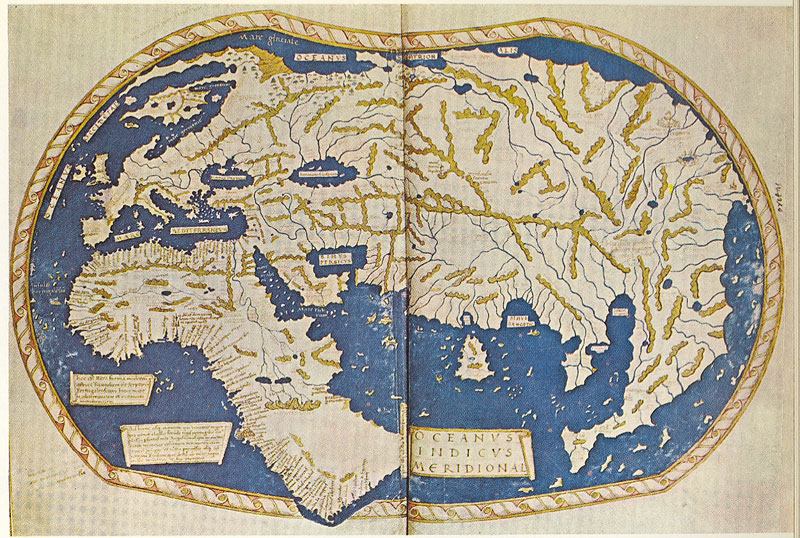
\includegraphics[width=100mm]{ge/worldMap1.jpg}
  \caption{Mapa świata z 1489 roku.}
  \label{fig:worldMap1}
\end{figure}

\chapter{Dostępne rozwiązania}
\label{sec:dostepnerozwiazania}

Przed rozpoczęciem implementacji własnego rozwiązania postanowiono przeprowadzić badania mające na celu analizę aktualnie dostępnych rozwiązań spełniających przynajmniej w części założenia. Proces ten nie ma na celu znalezienie idealnego rozwiazania lecz poznanie różnych podejść do zagadnienia, analiza różnych technologi które mogą być wykorzytane pozwoli na świadome wybranie najlepszych. 


\section{Google Earth}
\label{sec:Google Earth}

Funkcjonalnośc interaktywnych map można znaleść w aplikacji stworzonej przez firmę Google. Program ten jest napisany przy użyciu języka C++, nie służy on do tworznia aplikacji mobilnych, dlatego nie został on wybrany jako kandydat do naszej pracy.

Wykorzystuje ono statyczne obrazy będące zdjęciami satelitarnymi dla obrazów w dużej wysokośći lub zdjęciami wykonanymi z pokładów samolotów. Pomimo duzej atrakcyjności ma ono bardzo ograniczoną możliwośći zmiany oglądanych danych, ograniczone do ilości wykonanych zdjęć, dodatkowo większość punktów najstarsze dane ma z lat 50 XX w.

Przykład takiej sytuacji został przedstawiony na rysunku \ref{fig:lasVegas1}, obraz terenu na którym powstanie miasto Las Vegas w roku 1950. Jak teren ten wyglądał w roku 1977 widzimy na rysunku \ref{fig:lasVegas2}, pomimo widocznych zmian teren ten nadal w dużym stopniu jest pustynny,dopiero na rysunku \ref{fig:lasVegas3} widzimy aktualny stan miasta.

Dzięki funkcji zmiany punktu i kąta patrzenia, pokazywania ciekawych miejsc czy chociażby włączania trybu w którym budynki nabierają formy przestrzennej, 3D, możemy poprzez zabawę i wirtualne wycieczki poszeżać naszą wiedzę o otaczającym nas świecie.


\begin{figure}[H]
  \centering
    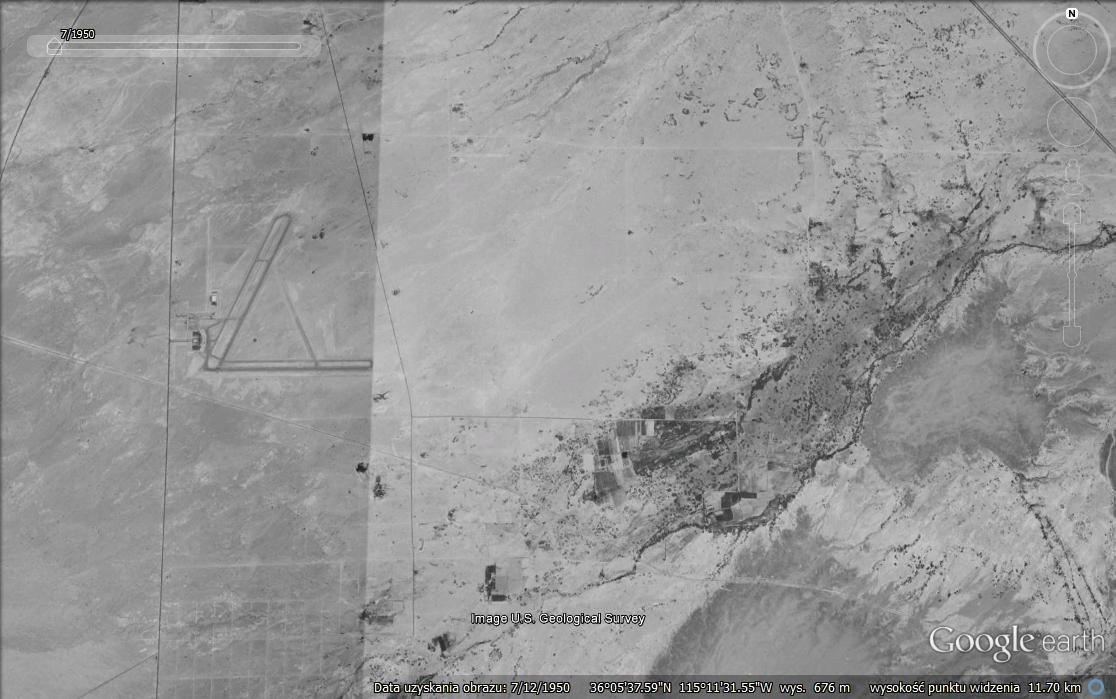
\includegraphics[width=100mm]{ge/01_1950.jpg}
  \caption{Las Vegas w 1950 roku.}
  \label{fig:lasVegas1}
\end{figure}

\begin{figure}[H]
  \centering
    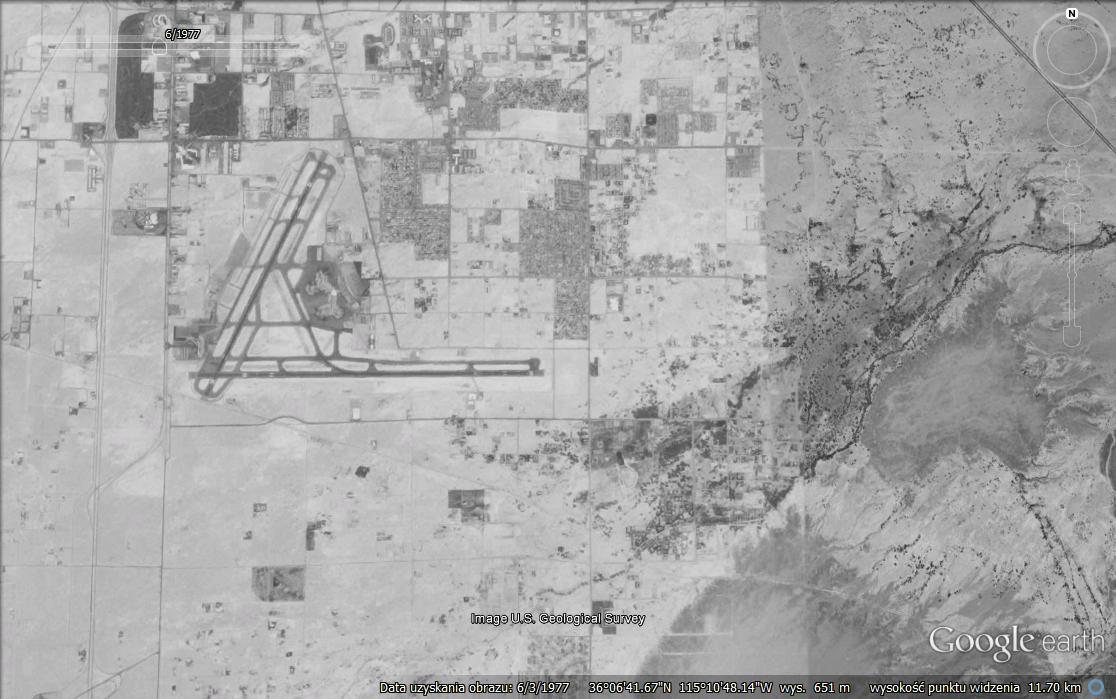
\includegraphics[width=100mm]{ge/02_1977.jpg}
  \caption{Las Vegas w 1950 roku.}
  \label{fig:lasVegas2}
\end{figure}

\begin{figure}[H]
  \centering
    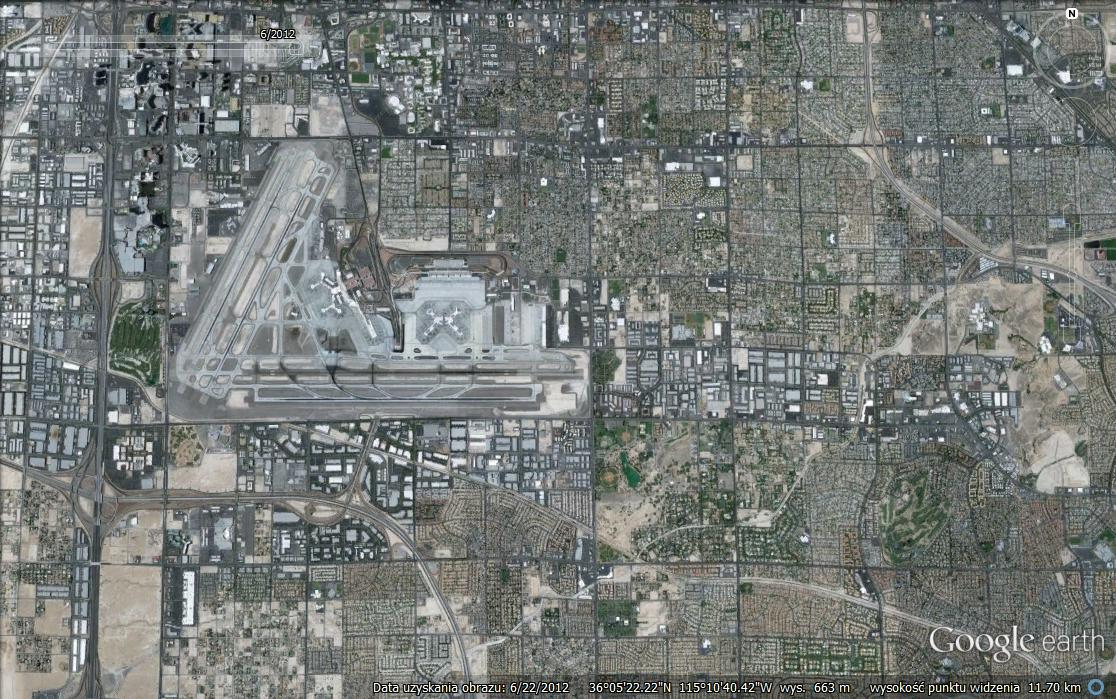
\includegraphics[width=100mm]{ge/03_2012.jpg}
  \caption{Las Vegas w 1950 roku.}
  \label{fig:lasVegas3}
\end{figure}




\chapter{Ogólny opis rozwiązania}
\label{cha:opis}

\section{Cel projektu}
\label{sec:celProjektu}

Celem projektu jest stworzenie aplikacji internetowej dodającej do tradycyjnych map dodatkowego wymiaru, czasu. Powinna dostarczać możliwości obserwowania zmian zachodzących na określonym terenie w danym okresie. Dodana oś czasu będzie miała za zadanie kontrolowanie okresu dla którego widoczne będą dane. Dostarczone dane przez użytkownika będą przedstawiane w czytelny i umożliwiający szybką analizę sposób. Przykładowe dane wejściowe to zmiany terytorialne w przeszłości, ukazanie rozowuju miast. Końcowa wizualizacja danych oprócz prostych kształtów geometrycznych musi zapewniać obsłógę zewnętrznych plików graficznych jak i najnowszych rozwiązań służących do obsługi grafiki.

\section{Problemy do rozwiązania}
\label{sec:problemy}

\begin{itemize}

\item
Przechowywanie i transmisja danych

Nie jest określony jeden format danych który będzie używany w aplikacji. Oprócz informacji opisujących położenie punktów zawarte również będą szczegółowe dane dotyczące ich wyglądu i zachowania, również obrazy graficzne mogą się znajdować w opisie mapy.

\item
Wizualizacja

Szeroki zakres informacji który może opisywać mapę musi być odpowiednio wyświetlany, w sposób czytelny i ułatwiający analizę dużych zbiorów danych. W jednym miejscu zostaną zebrane różnego rodzaju dane które muszą współpracować ze sobą tworząc spójną kompozycję.

\item
Bezpieczeństwo

Dane dostarczane przez zewnętrzny serwer powinny być wiarygodne. Użytkonwik posiadający kopię pliku znajdującą się na dysku lokalnym z infromacjami o mapię musi mieć możwliwość sprawdzenia jej autentyczności z aktualną wersją na serwerze.

\item
Optymalizacja rozwiązania

Aplikacja musi w każdym momencie zapewniać płynną pracę. Praca  ze szczegółową mapą posiadającą wiele informacji musi przebiegać płynnie, bez dużych opóźnień.

\end{itemize}

\section{Użytkownicy}
\label{sec:uzytkownicy}

\begin{itemize}
\item
Administrator

Osoba która posiada dostęp do serwera na krórym działa aplikacja korzystająca z omawianego frameworku. Ponieważ tworzony program jest jedynie narzędziem służącym do pracy z mapami, a jednym z założeń jest jak największa adaptowalność i możliwość działania na różnych środowiskach wymagana jest osoba która skonfiguruje współpracę z zewnętrzną stroną.

\item
Moderator

Pzygotowanie i edycja map powinna być wykonana przez uprawnione osoby. Może to być na przykład osoba posiadającą dużą wiedzę na dany temat, posiada ona możliwość edycji mapy.
\item
Uczeń

Użytkownik z najmniejszymy uprawnieniami, jedynie do przeglądania mapy.
\end{itemize}

\section{Granice systemu}
\label{sec:granicesystemu}

System umożliwia moderatorowi:
\begin{itemize}
\item
Tworzenie i edycję zestawów danych przechowywanych na serwerze

\item
Tworzenie własnych filtrów edytujących mapę w zależności od zmiany położenia lub czasu

\item
Zapis informacji o mapie do pliku na dysku lokalnym

\end{itemize}

System umożliwia uczniowi:
\begin{itemize}
\item
Przeglądanie gotowych map

\item
Pracę bez konieczności stałego dostępu do internetu.

\item
Sprawdzanie autentyczności pliku 

\end{itemize}

System nie umożliwia:
\begin{itemize}
\item
Wykorzystywania plików video

\end{itemize}

\section{Lista możliwości}
\label{sec:listamozliwosci}

Praca z mapami w trybie offline
\begin{itemize}
\item
Wczytywanie pliku - dane używane w aplikacji mogą zostać wczytane z dwóch źródeł. Z lokalnego dysku lub zaimportowane z serwera.

\item
Przechywanie danych po stornie klienta

\end{itemize}

Szeroki wachlarz dostęnych sposobów wizualizacji danych
\begin{itemize}
\item
Korzystanie z grafiki wektorowej

\item
Współpraca z plikami graficznymi

\item
Obsługa animacji poprzez svg

\end{itemize}

Współpraca z zewętrznymi aplikacjami
\begin{itemize}
\item
Obłsuga plików GML

\item
Parsowanie danych z formatu xml to pamięci storage

\end{itemize}

Tworzenie interaktywnych filtów
\begin{itemize}
\item
Filtry obsługjące zminę czasu

\item
Filtry obsługujące zmianę mapy

\end{itemize}


\section{Specyfikacja wymagań}
\label{sec:specyfikacja wymagan}

\subsection{Ogólny diagram przypadków użycia}
\label{sec:diagramcaseuse}


\begin{center}
\begin{figure}[H]
\centering
     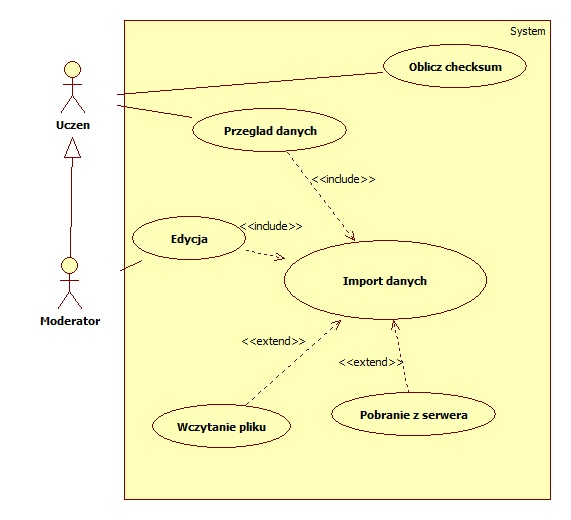
\includegraphics[origin=c,width=130mm]{ge/caseuse.jpg}
      \caption{Case use.}
       \label{fig:caseuse}
\end{figure}
\end{center}

\subsection{Definicje przypadków użycia}
\label{sec:defCaseuse}

Poniżej znajduje się opis trzech podstawowych przypadków użycia występujących w aplikacji. Opisane zostały warunki rozpoczęcia każdego z nich i ich zakończenia, zarówno pozytywnego jak i negatywnego.

\begin{table}[H]
    \centering
    \begin{tabular}{|l<{\raggedright}|p{3in}|}
    \hline
    Nazwa przypadku uzycia & Wczytanie danych z pliku  \\ \hline
    Typ przypadku uzycia  & Ogólny  \\ \hline
    Aktorzy   & Uczeń    \\ \hline
    Warunki wstepne   & Brak     \\ \hline
    Warunku koncowe dla sukcesu   & Dane zostaja zapisane w pamieci lokalnej przegladarki    \\ \hline
    Warunki koncowe dla niepowodzenia   & Dane nie sa poprawnie odczytane.     \\ \hline
    Scenariusz glówny   &

    \begin{enumerate}
    \itemsep0em
        \item Użytkownik wybiera plik.
        \item Dane podlegaja parsowaniu.
        \item Poprawnie odczytane dane zostaja zapisane w Storage.
    \end{enumerate}
     \\ \hline
    Scenariusz alternatywny   &

    \begin{enumerate}
    \itemsep0em
        \item Użytkownik wybiera plik.
        \item Dane podlegaja parsowaniu.
        \item Dane nie zostają odczytane poprawnie.
        \item Uzytkownik zostaje poinformowany o zainstniałym błędzie.
    \end{enumerate}
         \\ \hline
    \end{tabular}
    \caption{Przypadek wczytania danych}
    \label{tab:caseuse1}
\end{table}

\begin{table}[H]
    \centering
    \begin{tabular}{|l<{\raggedright}|p{3in}|}
    \hline
    Nazwa przypadku użycia & Wyświetlenie danych \\ \hline
    Typ przypadku użycia  & Ogólny  \\ \hline
    Aktorzy   & Uczeń     \\ \hline
    Warunki wstępne   & Dane znajdują się w pamięci lokalnej     \\ \hline
    Warunku końcowe dla sukcesu   & Dane zostają wyświetlone     \\ \hline
    Warunki końcowe dla niepowodzenia   & Mapa nie jest aktualizowana     \\ \hline
   Scenariusz glówny   &

    \begin{enumerate}
    \itemsep0em
        \item Użytkownik wybiera punkt w czasie.
        \item Dane dla wybranego okresu zostają wyrenderowane i pokazane.
        \item Informacje dla najbliższego otoczenia podlegają generacji i ukryciu.
    \end{enumerate}
     \\ \hline
    Scenariusz alternatywny   &

    \begin{enumerate}
    \itemsep0em
        \item Użytkownik wybiera punkt w czasie.
        \item Dane dla wybranego okresu nie zostają odnalezione
        \item Nie aktualne dane zostają schowane.
    \end{enumerate}
         \\ \hline
    \end{tabular}
    \caption{Przypadek wyświetlenia danych}
    \label{tab:caseuse2}
\end{table}

\begin{table}[H]
    \centering
    \begin{tabular}{|l<{\raggedright}|p{3in}|}
    \hline
    Nazwa przypadku użycia & Walidacja autentyczności pliku  \\ \hline
    Typ przypadku użycia  & Ogólny  \\ \hline
    Aktorzy   & Uczeń    \\ \hline
    Warunki wstępne   & Uczeń posiada plik na dysku i jego sumę kontrolną z serwera    \\ \hline
    Warunku końcowe dla sukcesu   & Pojawienie się komunikatu o autentyczności pliku    \\ \hline
    Warunki końcowe dla niepowodzenia   & Ostrzeżenie o dokonaniu zmian w pliku     \\ \hline
   Scenariusz glówny   &

    \begin{enumerate}
    \itemsep0em
        \item Użytkownik wybiera zakładkę do walidacji pliku.
        \item Podanie ścieszki do pliku i sumy kontolnej.
        \item Obliczenie aktualnej sumy dla pliku i porównanie go z podanym.
        \item Uzytkownik zostaje poinformowany o poprawności pliku.
    \end{enumerate}
     \\ \hline
    Scenariusz alternatywny   &

    \begin{enumerate}
    \itemsep0em
        \item Użytkownik wybiera zakładkę do walidacji pliku.
        \item Podanie ścieszki do pliku i sumy kontolnej.
        \item Obliczenie aktualnej sumy dla pliku i porównanie go z podanym.
        \item Użytkownik zostaje poinformowany o zmianach w pliku.
    \end{enumerate}
         \\ \hline
    \end{tabular}
    \caption{Przypadek kontroli pliku}
    \label{tab:caseuse2}
\end{table}

\subsection{Wymagania niefunkcjonalne}
\label{sec:niefunkcjonalnes}

Oprócz wymagań dotyczących prawidłowego funkcjonowania aplikacji, wymagane jest
aby zapewnione były poniższe punkty.

\begin{itemize}
\item
System powinien być skalowalny, powinien umożliwiać dostęp wielu użytkownikom równocześnie przy zachowaniu wymagań wydajnościowych.

\item
Aplikacja powinna działać identycznie na różnych środowiskach i przeglądarkach internetowych.
\end{itemize}

%\chapter{State of art}
\label{cha:State of art}
20-30
W rozdziale tym przedstawiono podstawowe informacje dotyczące struktury prostych plików \LaTeX a. Omówiono również metody kompilacji plików z zastosowaniem programów \emph{latex} oraz \emph{pdflatex}.

%---------------------------------------------------------------------------

\section{Rodzaje map}
\label{sec:Rodzaje map}

Tworząc aplikację która ma dostarczać informacji korzystających z map należy zapoznać się dostępnymi źródłami. Z powodu szrokiego wyboru poniżej omówione zostaną jedynie aplikacje które dostarczają informacji ogólnoświatowych. Na polskim rynku dostępnych jest kilka rozwiązań, ich główną wadą jest ograniczenie do terytorium Polski, dodatkowo często nie dostarczają one obrazów satelitarnych, są to m.in. \underline{\texttt{http://zumi.pl}}

\subsection{Google Maps}
\label{subsec:Google Maps}

\subsection{Windows Maps}
\label{subsec:Windows Maps}

\subsection{Apple Maps}
\label{subsec:Apple Maps}

\section{Google Earth}
\label{sec:Google Earth}

Ciekawe wykorzystanie obrazów satelitarnych i wskaźnika czasu zostało zaprezentowane w programie Google Earth. W aplikacji tej możemy zobaczyć nie tylko najbardziej aktualne zdjęcia, ale jesteśmy w stanie cofnąć się w czasie i zobaczyć jak wyglądał obszar na który patrzymy w przeszłości.

Przykład takiej sytuacji został przedstawiony na rysunku \ref{fig:lasVegas1}, obraz terenu na którym powstanie miasto Las Vegas w roku 1950. Jak teren ten wyglądał w roku 1977 widzimy na rysunku \ref{fig:lasVegas2}, pomimo widocznych zmian teren ten nadal w dużym stopniu jest pustynny,dopiero na rysunku \ref{fig:lasVegas3} widzimy aktualny stan miasta.

Dzięki funkcji zmiany punktu i kąta patrzenia, pokazywania ciekawych miejsc czy chociażby włączania trybu w którym budynki nabierają formy przestrzennej, 3D, możemy poprzez zabawę i wirtualne wycieczki poszeżać naszą wiedzę o otaczającym nas świecie. 

\begin{figure}[H]
  \centering
    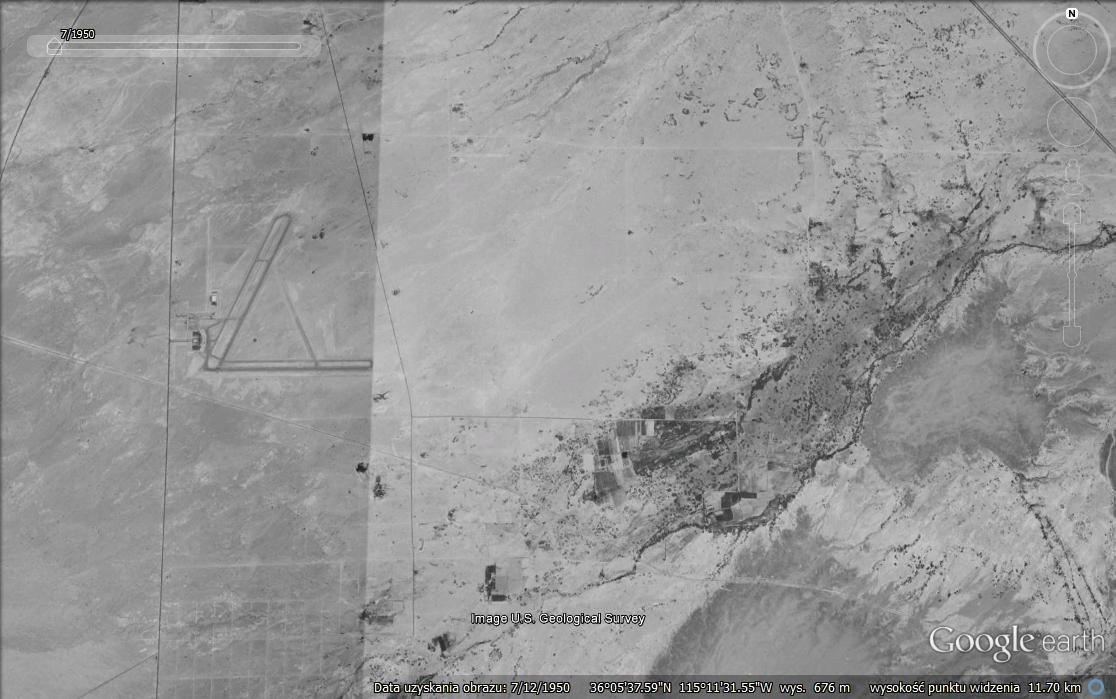
\includegraphics[width=100mm]{ge/01_1950.jpg}
  \caption{Las Vegas w 1950 roku.}
  \label{fig:lasVegas1}
\end{figure}

\begin{figure}[H]
  \centering
    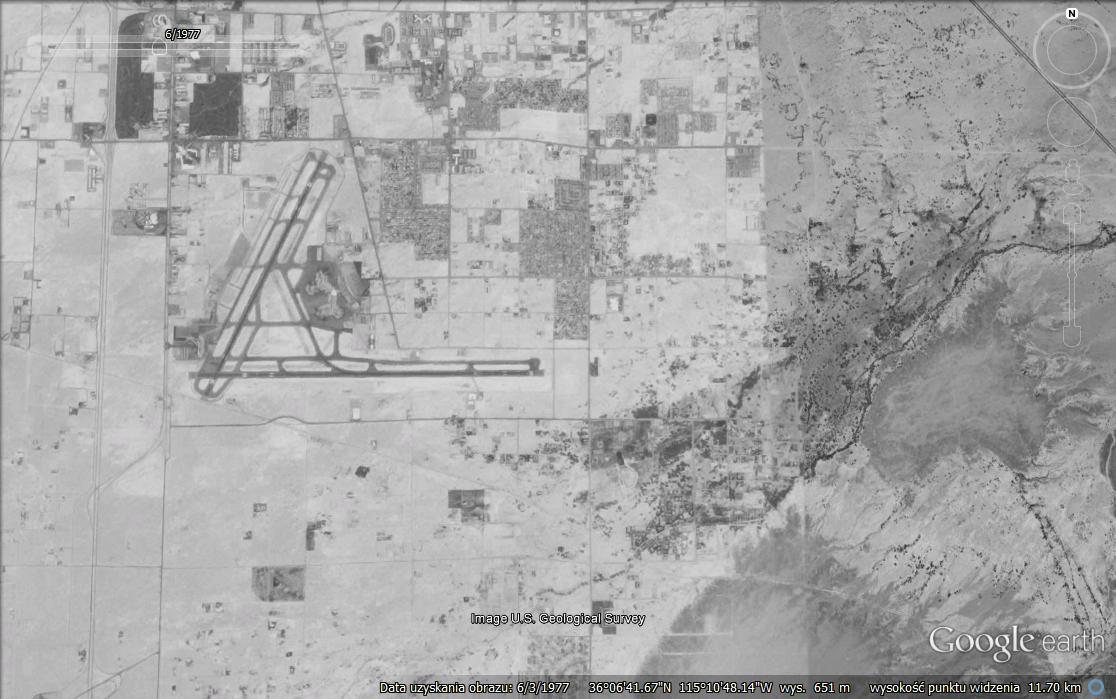
\includegraphics[width=100mm]{ge/02_1977.jpg}
  \caption{Las Vegas w 1950 roku.}
  \label{fig:lasVegas2}
\end{figure}

\begin{figure}[H]
  \centering
    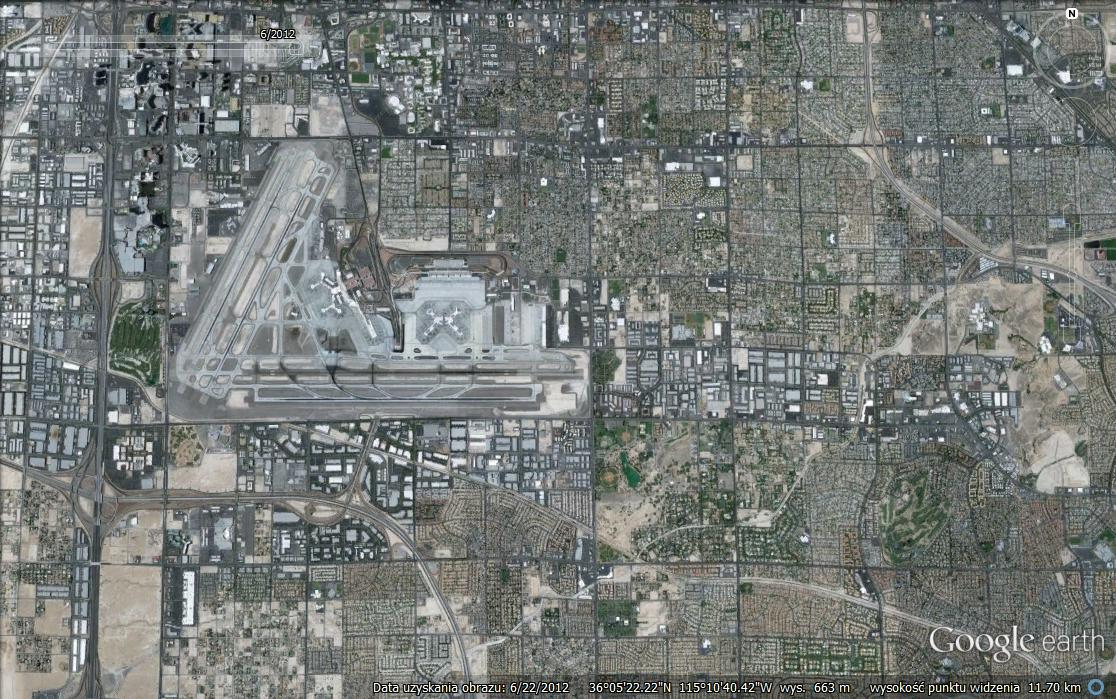
\includegraphics[width=100mm]{ge/03_2012.jpg}
  \caption{Las Vegas w 1950 roku.}
  \label{fig:lasVegas3}
\end{figure}

\section{Time line}
\label{sec:Time line}

Plik \LaTeX owy jest plikiem tekstowym, który oprócz tekstu zawiera polecenia formatujące ten tekst (analogicznie do języka HTML). Plik składa się z dwóch części:
\begin{enumerate}%[1)]
\item Preambuły -- określającej klasę dokumentu oraz zawierającej m.in. polecenia dołączającej dodatkowe pakiety;

\item Części głównej -- zawierającej zasadniczą treść dokumentu.
\end{enumerate}


\begin{lstlisting}
\documentclass[a4paper,12pt]{article}      % preambuła
\usepackage[polish]{babel}
\usepackage[utf8]{inputenc}
\usepackage[T1]{fontenc}
\usepackage{times}

\begin{document}                           % część główna

\section{Sztuczne życie}

% treść
% ąśężźćńłóĘŚĄŻŹĆŃÓŁ

\end{document}
\end{lstlisting}

%---------------------------------------------------------------------------

\section{Kompilacja}
\label{sec:kompilacja}

\begin{lstlisting}
latex test.tex
dvips test.dvi -o test.ps
ps2pdf test.ps
\end{lstlisting}
%
lub za pomocą PDF\LaTeX:
\begin{lstlisting}
pdflatex test.tex
\end{lstlisting}

%---------------------------------------------------------------------------

\section{Narzędzia}
\label{sec:narzedzia}

\begin{itemize}
\item Edit shortcuts -- definiowanie własnych klawiszy skrótu;
\item Line Tools -- dodatkowe operacje na liniach tekstu;
\end{itemize}

%---------------------------------------------------------------------------

\section{Przygotowanie dokumentu}
\label{sec:przygotowanieDokumentu}

Plik źródłowy \LaTeX a jest zwykłym plikiem tekstowym. Przygotowując plik
źródłowy warto wiedzieć o kilku szczegółach:

\begin{itemize}
\item
Poszczególne słowa oddzielamy spacjami, przy czym ilość spacji nie ma znaczenia.
Po kompilacji wielokrotne spacje i tak będą wyglądały jak pojedyncza spacja.
Aby uzyskać {\em twardą spację}, zamiast znaku spacji należy użyć znaku {\em
tyldy}.

\item
Znakiem końca akapitu jest pusta linia (ilość pusty linii nie ma znaczenia), a
nie znaki przejścia do nowej linii.

\item
\LaTeX~sam formatuje tekst. \textbf{Nie starajmy się go poprawiać}, chyba, że
naprawdę wiemy co robimy.
\end{itemize}



\chapter{Opis rozwiazania}
\label{cha:problem}

Poniższy rozdział zawiera omówienie technologi które zostały wykorzystane w procesie tworzenia aplikacji, ze szczególnym uwzględnieniem funkcjonalności które okazały się najbardziej przydatne. Następnie zawarto szczegółowy opis sposóbów rozwiązania problemów które należało rozwiązać w trakcie tworzenia interaktywnej mapy.

\section{Wykorzystane technologie}
\label{sec:wykorzystanetechnologie} 

\subsection{JavaScript}
\label{sec:javascript}

Wybór języka JavaScript to tworzenia aplikacji został podyktowany jego dużymi możliwościami na polu tworzenia projektów do użytku na przeglądarkach internetowych.Pozwala na łatwe tworzenie asynchronicznych aplikacji, oznacza to aktualizowanie jedynie wybranych danych na ekranie moniotra bez konieczności przeładowania całej strony. Jest to szczególnie istotne w omawianym przypadku, oznacza to brak potrzeby wczytywania i renderowania całego tła mapy za każdym razem gdy nastąpi nawet małą zmiana.


Spełnia warunki paradygmatu obiektowego, umożliwia korzystanie z obiektów które mogą odpowiadać pewnej klasie rzeczywistych przedmiotów lub rzeczy, imperatywnego, składa się z komend które zmieniają stan programu jak też funkcyjne, umożliwia tworzenie funkcji które w zależności od podanych argumentów wejściowych dostarczają odpowiednich danych wyjściowych.

Bardzo ważną cechą języka jest fakt jego wykonywania po stronie klienta. Oznacza to wykonywanie obliczeń i korzystanie z pamięci najczęściej na komputerze osoby która korzysta z aplikacji. Pozwala to na zmiejszenie wymagać w stosunku do serwera( wykonyje on mniej operacji i zapisuje mniej danych w swojej pamięci)

Obecnie powstają frameworki których zadaniem jest stworzenie małej, lekkiej aplikacji webowej wykorzystującej w maksymalny sposób omawiany język.\cite{AngularJS} Przykładem takiego rozwiązania jest AngularJs, korzysta on z architekury MVC w której większość pracy została przeniesiona na stronę klienta. Kontroler wykonuje obliczenia w przeglądarce użytkownika, odciąża to główny serwer, pozwala na szybszą i płynniejszą pracę większej ilości osób.

Nie wątpliwą zaletą takiego podejścia jest wzrost opdorności na ataki typu Dos(en. Denial of Service), polega on na przeciążeniu aplikacji dostarczającej określone dane lub usługi do momentu gdy przestaje ona opdowiadać na jakiekolwiek zapytania. Aplikacje które wykonują większość operacji po stronie serwera(różnego typu obliczenia matematyczne, analizę danych) aby sprostać dużej ilośći klientów która występuje w tego typu atakach nakłada duże wymagania w stosunku do wykorzystywanego sprzętu elektrycznego. Przeniesienie ciężaru z serera na końcowego klienta wykonywania większości operacji pozwala nie tylko na obsłużenie większej ilości użytkowników ale także może wpłynąć na zmiejszenie kosztów utrzyamnia serwera.

Prosty przykład na stronie \underline{\texttt{http://angularjs.org/}} prezentuje w jak prosty sposób można stworzyć prostą liste rzeczy do zrobienia. Poniżej zaprezentowano fragment odpowiedzialny za wyświetlenie zadań z dodatkowym polem określającym czy zostało już wykonane.

\lstset{language=JavaScript}
\begin{lstlisting}[caption=AngularJs]

        //fragment kodu html
      <div ng-controller="TodoCtrl">
        ...
        <li ng-repeat="todo in todos">
          <input type="checkbox" ng-model="todo.done">
          <span >{{todo.text}}</span>
        </li>
        ...
      </div>

        //kontroler
        function TodoCtrl($scope) {
          $scope.todos = [
            {text:'learn angular', done:true}];
          ...
        }
\end{lstlisting}

\subsection{Możliwości HTML5}
\label{sec:html5}
\nocite{xml50}
\nocite{proxml}
\nocite{pre1}
\nocite{pre2}
\nocite{googlemapsbegin}
\nocite{proHTML5}
HyperText Markup Language,  hipertekstowy język znaczników
Pozwala na opisanie struktury informacji zawartych na stronie internetowej, to dzięki niemu przeglądarka moze rozróżnić takie elementy jak hiperłącze, akapit czy chociażby nagłówek.

Podobnie jak w przypadku XML, tak i tutaj wymagane jest aby wykorzystywane znaczniki umieszczane były w nawiasach ostrokątnych, a każdy z nich miał swoje domknięcie.

Poprawnym zapisem jest <p>Wiadomość<\textbackslash p> który oznacza pojedyńczy akapit. Zapis <p>Wiadomość<p>, który różni się od poprzedniego brakiem znaku "\textbackslash" w drugim znaczniku, czyni to ten zapis niepoprawnym. Istnieje możliwość aby wykorzystać pojedyńczy znacznik, przykładem jest <br \textbackslash> określający wstawienie nowej lini w miejscu wystąpienia tagu.

Obecnie powszechnie używany standart HTML4 ma niestety wiele ograniczeń, z tego powodu pracowano nad jego następnikiem. 22 stycznia 2008 W3C opublikował HTML5, wtedy jeszcze jako jedynie szkic.


\subsection{Less}
\label{sec:less}

Do stworzenia bardziej zaawansowanych arkuszy stylów CSS (en. Cascading Style Sheets) wykorzystaniu narzedzie które pozwala na łatwe tworzenie i utrzymywanie reguł. Głównymi zaletami są:

\begin{itemize}
\item
Deklarowanie zmiennych.

Jeśli chcemy wykorzystać jedną wartość(przykładowo jeden kolor) w wielu miejscach wystarczy w głównym pliku zadeklarować zmienną i wykrzystywać ją w każdym miejscu gdzie chcemy użyć tej wartośći.

Przykładowo chcąc wykorzystać kolor czerwony wykorzystywany w kolorystyce uczelni AGH deklarujemy zmienną @aghRed, następnie w miejscu gdzie chcemy aby pojawił się ten kolor korzystamy z istniejącej zmiennej

\lstset{language=JavaScript}
\label{lis:webSql}
\begin{lstlisting}[caption=json]
@aghRed: #a71930;
bgcolor: @aghRed;
\end{lstlisting}

\item
Mixiny

Możemy tworzyć nowe klasy które będą posiadały właściwości innej, wcześniej zadeklarowanej.Pozwala to na tworzenie kodu bardziej czytelnego, niepowielanie go.


\lstset{language=JavaScript}
\label{lis:webSql}
\begin{lstlisting}[caption=json]
.RoundBorders {
  border-radius: 5px;
  -moz-border-radius: 5px;
  -webkit-border-radius: 5px;
}
#menu {
  color: gray;
  .RoundBorders;
}
\end{lstlisting}

\item
Osadzanie elementów wedlug dziedziczenia

Tworząc zagnieżdzoną strukturę storny często elementy wewnętrzne zależą od elementów nadrzędnych. Wygląd komurki może się różnić w zależości od rodzaju tabeli. W tworzeniu tak zadnieżdżonych struktur pomocna okazuje się omawiana cecha.

\end{itemize}

\clearpage
\newpage
\section{Przechowywanie i transmisja danych}
\label{sec:przesyl}

\subsection{GIS}
\label{subsec:gis}

GIS(Geographical Information Systems) jest to System Informacji Geograficznych, połącznie danych i technologi aby dokonywać pomiarów, analizy i przedstawiania danych związanych z informacjami geograficznymi. Dane są pobieranie w trakcie naziemnych pomiarów jak i zbierane przy użyciu sztucznych satelitów. Informacje te są następnie zapisywane do określonych formatów dzięki czemu możliwe jest ich dalsze przetwarzanie.

\subsubsection{Wykorzystywany układ współrzędnych}
\label{subsec:uklad}

Istnieje wiele układów współrzędnych które służą do opisu pojedyńczego punktu na powierzchni ziemi. Na stronie \underline{\texttt{http://www.spatialreference.org/ref/epsg/}} (dostęp 20.11.2013) znajduje się lista zawierająca przykłady zapisu punktu na kuli ziemskiej przy użyciu różnych formatów, zawierają one niezbędne infomacje do poprawnego zapisu danych w określonym formacie.

Tradycyjny zapis oparty jest na wykorzystaniu stopni, minut i sekunk, jest on obecnie wypierany przez nowszy, łatwiejszy do obliczeń komputerowych. Wersją która ma za zadanie być ogólnoświatowym formatem jest WGS(World Geodetic System). Jego ostatnia wersja  WSG84 jest powszechnie używana w urządzeniach do nawigacji. Poniżej zaprezentowano jak wygląda zapis w starszym i nowszym punktu określającego położenie budynku A-0 uczelni AGH.

\begin{itemize}

\item
Pierwotny zapis

50°03'52.2803", 19°55'23.7968"
\item
Zapis unowocześniony

50.06452231874906, 19.923276901245117
\end{itemize}

Drugi zapis został wykorzystany do przechowywania danych w plikach, tak aby wymiana i wspólna praca była jak najprostsza. Wybór ten sprawił że nie występuje problem konwersji punktu do formatu czytelnego dla komputera, można go bez problemu odczytać jako liczbę.

\subsection{Format zapisu}
\label{subsec:zapisWektorowy}

W celu przechowywania obiektów graficznych zdecydowano się na wykorzystanie grafiki wektorowej. Oprócz bezproblemowej skalowalności, pozwala ona również na szeroką i łatwą edycję.
Obraz jest w tym przypadku przechowywany jako zbiór formuł matematycznych m.in. proste i łuki. Dzięki takiemu podejściu obraz w dowolnej skali na identyczną jakość, widać to na rysunku \ref{fig:wekt}. Przykładowymi formatami są GML(Geography Markup Language) otwarty standart XML dla wymiany danych GIS, Shapefile czy tradycyjny kartezjański układ współrzędnych.

  \begin{figure}[H]
  \centering
    
\includegraphics[width=50mm]{ge/a1.jpg}
  \caption{Zapis wektorowy}
  \label{fig:wekt}
  \end{figure}

Przeciwnym podejściem jest grafika rastrowa, jest to zapis punktów o określonym kolorze i położeniu na płaszczyźnie.  Efektem takiego podejścia jest pogorszenie obrazu w momencie dużego powiększenia. Przykładem są formaty takie jak ADRG,ASC czy RGB.
Porównanie litery "S" i jej 7-krotnego powiększenia w tym zapise zaprezentowano na rysunku \ref{fig:rast}
  \begin{figure}[H]
  \centering
    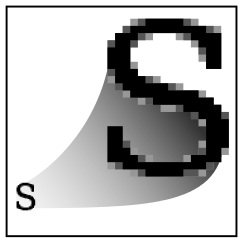
\includegraphics[width=50mm]{ge/a2.jpg}
  \caption{Zapis rastrowy}
  \label{fig:rast}
  \end{figure}

\subsection{Format pliku}
\label{subsec:fileformat}

W celu wypełnienia założeń projektu jakim jest umożliwienie przechowywania danych w zewnętrznym pliku przeprowadzono analizę dostępnych formatów zapisu danych kartograficznych.

\begin{itemize}

\item
SWDE(Standard Wymiany Danych Ewidencyjnych) - polski format służący głównie do wymiany danych ewidencyjnych gruntów i budynków

\item
SWING(Standard Wymiany INformacji Geodezyjnych) - format danych geodezyjnych służący do wymiany danych pomiędzy bazami danych systemów informatycznych SIT(wikipedia.pl)

\item
KML(Keyhole Markup Language) - otwarty standart oparty na XML-u, stworzony głównie dla potrzeb GoogleEarth

\item
GML(Geography Markup Language) - stworzony przez OGC(Open Geospatial Consortium) międzynarodową organizację założoną w celu tworzenia i rozpowszechniania standarów związanych z informacjami dotyczącymi geograficznych i geoprzestrzennych danych

\end{itemize}

Dwa polskie formaty są stosunkowo mało popularne, są one głównie wykorzystywane w celu komunikacji pomiędzy rządowymi bazami danych. Zawierają one bardzo określone typy danych co sprawia że są mało przydatne dla ninijeszego projetku. KML jest formatem który posiada szeroki wachlarz dostępnych znaczników a jego duża popularność dostarcza dużą bazę plików gotowych do wykorzystania. Niestety został on stworzony by współpracować z określonym programem, zaimplementowane zostały jedynie elementy które mogą zostać wykorzystane w nim. Ostatni przykład został stworzony w uniwersalnym celu do ogólnego użytku, posiada on bardzo dużo możliwości, apadtacji do konkretnych rozwiązań\cite{gml} z uwagi na ten fakt zdecydowano się na wybór tego rozwiąznia. Nie zostaną wykorzystane jego pełne możliwości, jedynie te które są przydatne w projektowanej aplikacji.
Jedną z ciekawych i przydatnych możliwości podczas jego wykorzystania jest zgodność z formatem KML na bazie którego powstało wiele zbiorów danych gotowych do wykorzystania.


\subsection{Pliki graficzne}
\label{subsec:plikigraficzne}

Obrazy graficzne które mogą wystąpić w zbiorze danych wejściowych zdecydowano się przechowywać w postaci osobnych plików, nie są one załączane do głównego. Są to pliki które mogą stanowić alternatywne tło mapy, lub fragment wzbogadzający wizualne dane.

Chcąc wykorzstać zasób zapisany w formaci jpg lub png należy w odpiednim znaczniku podać jego ścieżkę względną lub bezwzględną w przypadku gdy znajduje się na komputerze użytkownika lub adres internetowy pod którym się znajduje.

Zaletami takiego podejścia jest:
\begin{itemize}

\item
Łatwa reużywalność zasobów graficznych, jeden plik może być wykorzystany przez kilka map bez potrzeby jego powielania.

\item
Dzięki separacji fragmentów alfanumerycznych od binarnych zachowana jest maksymalna czytelność danych.

\end{itemize}

\subsection{Parser plików}
\label{subsec:parser}

Założenia projektu zakładają dostarczanie wstępnego zestawu danych opisujących mapę poprzez plik tekstowy zawierający dane w określonym formacie. Może on znajdować się na zewnętrznym serwerze lub dysku lokalnym. W pierwszym przypadku zostanie on najpierw ściągnięty do pamięci lokalnej aby następnie mógł być wykorzystany, w drugim po podaniu ścieżki dostępu do niego  od razu nastąpi jego analiza. Aby było to możliwe stworzony został parser którego zadaniem jest odczytanie danych i przygotowanie ich aby możliwe było ich wykorzystanie w dalszej pracy aplikacji.

Wybrany format danych wybrany podczas prac badawczych, GML, zawiera bardzo obszerny zbiór elementów pozwalających opisywać bardzo szeroki wachlarz obiektów, takich jak mosty, budynki pojazdy. Taka dokładność nie jest wymagana w tym przypadku z tego powodu parser nie obsługuje całego języka. 

Ponieważ można przygotować plik w formacie GML w taki sposób aby przypominał zapis KML zdecydowano się zwrócić szczgólną uwagę aby parser poprawnie rozpoznawał i dekodował dane również z tej postaci, pozwoli to na dostęp do dużej bazy gotowych informacji.
Wczytane informacje podlegają przetworzniu ze składni XML, na którym bazuje GML do notacji JSON która jest używana podczas pracy map.

\subsection{Storage}
\label{subsec:storage5}
Aby stworzyć framework który będzie w stanie działać przy minimalnej konieczności konfiguracji dodatkowych środowisk postanowiono aby dane w pierwszej kolejności były przechowywane po stronie klienta. Do tego celu nadaje się funkcjonalność stworzona w ostatniej wersji HTML którą jest Storage. Pozwala on na przechowywanie danych w przeglądarce użytkownika \cite{html5dive}. Różnicą w stosunku do ciasteczek które również potrafią przechowywać dane są:
\begin{itemize}
\item
Większy rozmiar dostępnej pamięci m.in. Chrome 5MB \nocite{chrome5mb}, IE 10MB
\item
Informacje przechowywane są po stronie użytkownka, nie są przesyłane za każdym razem do serwera.
\item
Informacja może być przechowywana przez długi okres czasu.
\end{itemize}

Wadą tego typu pamięci jest jej interfejs. Obecnie przechowywany sposób danych to mapowanie w postaci napis->napis. Wymusza to aby dane które chcemy przechować były zapisane jako ciągi znaków. Przykład \ref{lis:Namestorage} przedstawia w jaki sposób możemy obiekt zawierający imię i nazwisko zapisać w pamięci. Linia 4 przedstawia obiekt w postaci której chcielibyśmy go przechować. Niestety zwykłe przypisanie do zmiennej w pamięci powoduje że jedynie typ instancji zostaje zapisany. Aby móc zapisać w poprawnej formie dane musimy doknać serializacji danych. Czynność tą możemy wykonać przy pomocy metody ``stringify'' z obiektu JSON, wynikiem jest ciąg znaków który możemy bez problemu zapisać w pamięci sesyjnej. Do odzyskania pierwotnego obiektu, odtworzenia go z zapisanego napisu wykorzystujemy metodę ``parse'' również z obiektu JSON.

Dodatkowo nie można pominąć faktu istnienia dwóch typów.
\begin{itemize}

\item
Session Storage

Dane przechowywane są w kontekście sesji użytkownika, są one tracone w momencie zamknięcia okna przeglądarki.

\item
Local Storage

Teoretycznie dane są przechowywane w nieskończoność, do momentu kiedy użytkonwik nie usunie ich. Zamknięcię sesji nie powoduje usunięcia danych.

\end{itemize}

Zapisywanie informacji po stronie klienta ma na celu zachowanie aktualnego stanu mapy, dokonanych zmian i naniesionych poprawek, informacje o poprzednich są zbędne. Sytuacja ta jednoznacznie wskazuje że lepszym wyborem jest pamięć sesyjna(Session Storage).

\lstset{language=JavaScript}
\label{lis:Namestorage}
\begin{lstlisting}[caption=Wykorzystanie Storage]
      uzytkownik={};
      uzytkonwik.imie='Jan'
      uzytkownik.nazwisko='Kowalski'
      //uzytkownik : Object {imie: "Jan", nazwisko: "Kowalski"}

      sessionStorage.u1 = uzytkownik
      //sessionStorage.u1 : "[object Object]"

      sessionStorage.u2 = JSON.stringify(uzytkownik)
      //sessionStorage.u2 : "{"imie":"Jan","nazwisko":"Kowalski"}"

      uzytkonwik2 = JSON.parse(sessionStorage.u2)
      //uzytkonwik2 : Object {imie: "Jan", nazwisko: "Kowalski"}
\end{lstlisting}


Podsumowanie dostępne na stornie \underline{\texttt{http://www.html5rocks.com/en/features/storage}} (dostęp 31.10.2013) pozwala na sprawdzenie minimalnej wersji przęglądarki od której wspierane jest to rozwiązanie. Wskazuje ono na największą dostępność spośród dostępnych sposobów przechowywania informacji po stornie klienta.

\subsection{Transmisja danych}
\label{subsec:transmisjaDanych}

Ważnym aspektem który należy rozwiązać jest sposób przesyłania danych. Problem ten jest szczególnie istotny w omawianej pracy z uwagi na możliwość przesyłania dużej ilości informacji o granicach lub innych liniach przezentowanych na mapie. Do opisu kwadratowego obszaru wymagane jest przesłanie informacji o minimum 4 punktach. Jeżeli będziemy chcieli przekazać dokłądniejszy zarys obszaru, zaprezentować granicę państwa lub linię frontu wojennego linia prosta w większości przypadków będzie zbyt ogólnym przybliżeniem, nie oddającym prawdziwej sytuacji.

Projekt zakłada korzystanie z lokalnej pamięci komputera użytkownika podczas pracy, jednak dostarczenie informacji, danych wejściowych nie powinno być ograniczone do wczytania ich z pliku tekstowego, należy pamiętać o możliwości przesłania ich z serwera aplikacji do użytkownika. W sytuacji takiej, gdzie w jednym momencie przesłane zostaną wszystkie informacje dotyczące mapy, ilość danych może być znaczna.

Z raportu Akamai wynika że śrenia przepływność łączy internetowych dla użytkowników korzystających z puli adresów IP przeznaczonych dla Polski w I kwartale 2012 r. wynosiła 5Mb/s  \underline{\texttt{http://www.rp.pl/artykul/924483.html}} (dostęp 13.10.2014). Jest to bardzo dobry wynik który plasuje Polskę w czołówce rankingu. Pomimo tego wyniku nie można pominąć faktu optymalizacji przesyłanych danych, wymieniane dane pomiędzy użytkownikiem a serwerem powinny być jak najmniejsze. Duża popularność urządzeń mobilnych w których dostęp do internetu jest zapewniany często poprzez sieć bezprzewodową a dostęp do interentu nie jest jeszcze tak dogodny jak jest to w przypadku użytkowników stacjonarnych  wymusza minimalizowanie przesyłanych informacji.

Kolejnym powodem dla którego odpowiedzi serwera powinny być jak najlżesze jest koszt pracy samego serwera. Jest to szczególnie widoczne w dużych aplikacjach mających wielu użytkowników, czas jaki jest przeznaczany dla pojedyńczego jest mnożony przez ich ilość. Z tego powodu zawsze podczas zwiększenia ilości użtkowników korzystających z aplikacji następuje zwiększenie stawianych wymagać wobec serwera, w ostateczności wymagane jest wykorzystanie kolejnej fizycznej maszyny. Celem programisty tworzącego kod który będzie wykorzystywał zasoby serwera(zarówno jego czas procesora jak i pamięć) jest dbanie aby moment w którym niezbędne będzie korzystanie z większej ilośći maszym nastąpił przy jak największej ilości użytkowników.

Z uwagi na omówione aspekty zdecydowano się aby w przypadku korzystania z danych nie znajdujacych się na lokalnym dysku komputera wszystkie infromacje dotyczące mapy zostały przesłane jako plik w określonym formacie. Zostanie on zapisany w pamięci komputera użytkownika i podlegał dalszej pracy. Takie podejście minimalizuje wymagania nakładane na serwer i czas zajęcia procesowa.

\newpage

\clearpage
\newpage
\section{Wizualizacja}
\label{sec:wizualizacja}

Poniższa sekcja zawiera próbę analizy dostępnych metod prezentacji danych zarówno zbiorów punktów, zdjęć jak i animacji. Główną uwagę zwrócono na 3 główne sposoby wizualizacji grafik. Ostatnia część zawiera zbiór dostępnych funkcjonalności, stanowi przewodnik po dostępnych możliwościach i ukazuje w jaki sposób można personalizować dane.


\subsection{Rodzaje map}
\label{subsec:Rodzaje map}

Tworząc aplikację która ma dostarczać informacji korzystających z map należy zapoznać się dostępnymi źródłami. Z powodu szerokiego wyboru poniżej omówione zostały jedynie aplikacje które dostarczają informacji ogólnoświatowych. Na polskim rynku dostępnych jest kilka rozwiązań, ich główną wadą jest ograniczenie terytorialne, dodatkowo często nie dostarczają one obrazów satelitarnych, przykładem jest zumi (\underline{\texttt{http://zumi.pl}}).

\subsubsection{Windows Maps}
\label{subsubsec:Windows Maps}

Rysunek \ref{fig:bingMaps_1} przedstawia obraz otrzymany wykorzystując Bing Maps. W tym konkretnym przykładzie widzimy znaczną różnicę kolorów, obecność chmur pomniejsza wartość tych zdjęć. Należy wspomnieć o ubogim interfejsie dostarczanym użytkownikowi.

\begin{figure}[H]
  \centering
    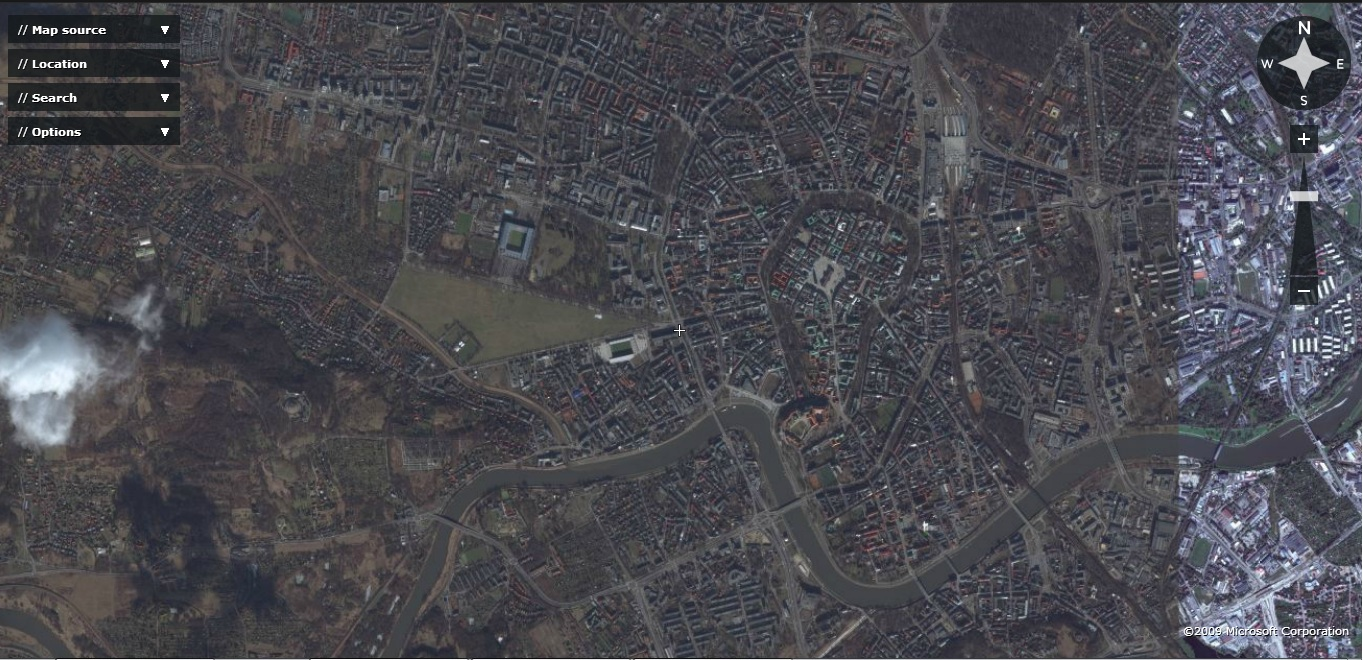
\includegraphics[width=100mm]{ge/bing_1.jpg}
  \caption{Bing Maps.}
  \label{fig:bingMaps_1}
\end{figure}

\subsubsection{Yahoo Maps}
\label{subsubsec:Yahoo Maps}

Kolejnym dostarczycielem danych kartograficznym jest Yahoo, przykład znajduje się na rysunku \ref{fig:yahooMaps_1}. Interfejs jest zbliżony do Bing Maps, jednak obszar na którym możemy przedlądać zdjęcia jest mniejszy, tereny oddalone od większych miast nie są w pełni uwzglęnione. Z tego powodu nie stanowi w pełni akceptowalnego rozwiązania.

\begin{figure}[H]
  \centering
    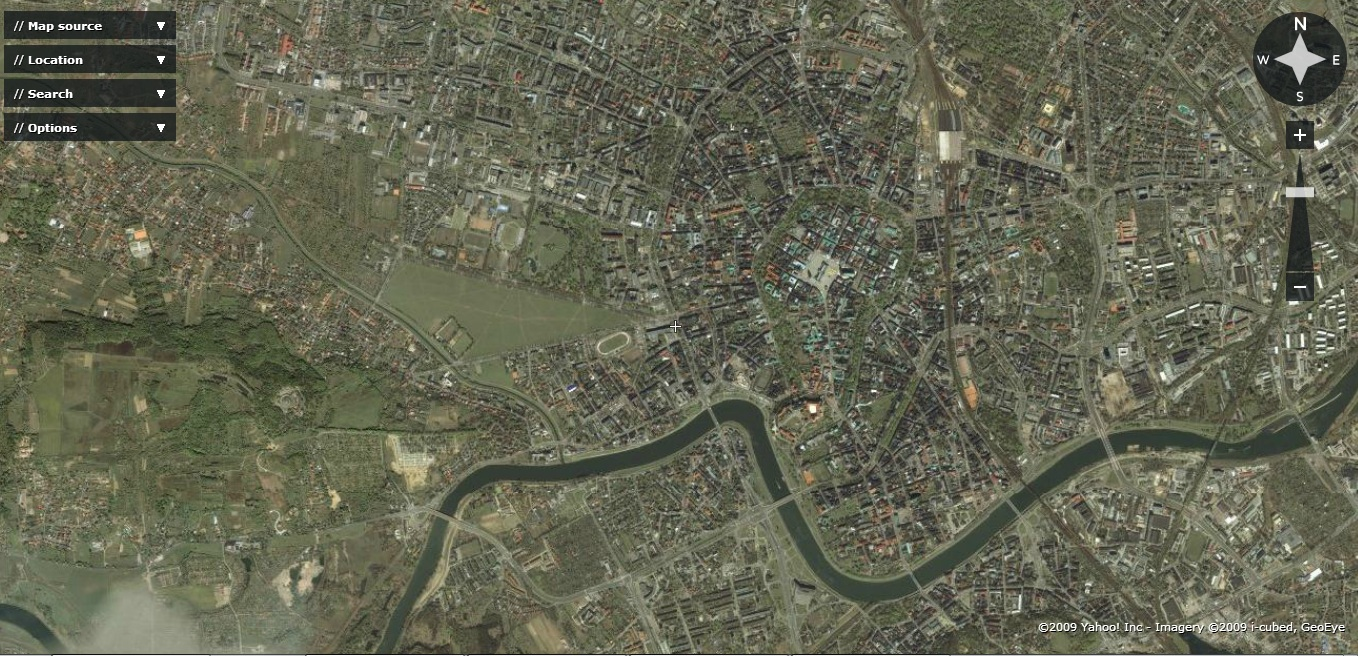
\includegraphics[width=100mm]{ge/yahoo_1.jpg}
  \caption{Yahoo Maps.}
  \label{fig:yahooMaps_1}
\end{figure}


\subsubsection{Apple Maps}
\label{subsubsec:Apple Maps}

Kolejną dużą marką która dostarcza informację jest Apple. Niestety nie ma wersji która pozwalałaby na dostęp do tej usługi z powszechnie używanych komputerów stacjonarnych. Dodatkowo jakość dostarczanych informacji jest złej jakości.

\subsubsection{Google Maps}
\label{subsubsec:Google Maps}
\nocite{googlemapsbegin}
Rysunek \ref{fig:googleMaps_1} przedstawia obraz otrzymany w aplikacji Google Maps. Dodatkowo włączona opcja prezentacji natężenia ruchu jedynie potwierdza duże możliwości i łatwość obsługi. Przyjazny interfejs sprawia że praca jest prosta i pozwala na osiągnięcie bardzo dobrych wyników. Z uwagi na wielkie korzyści i duże możliwości konfiguracji rozwiązanie to zostało wybrane jako bazowe w tworzonej pracy.


\begin{figure}[H]
  \centering
    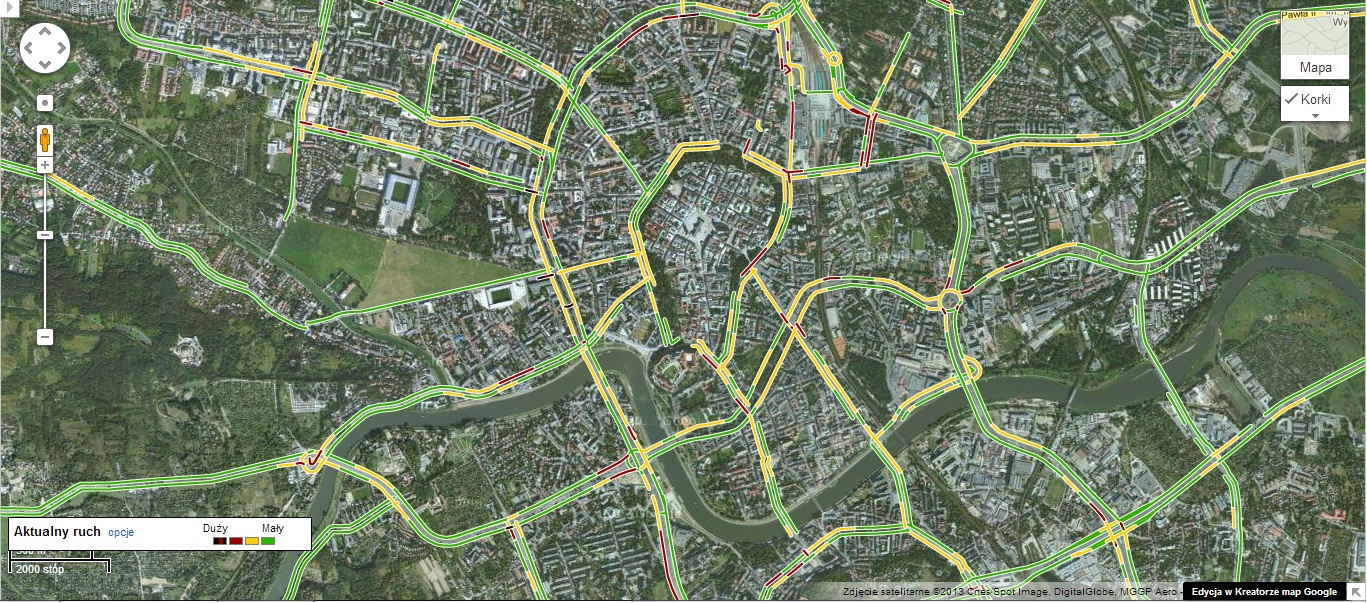
\includegraphics[width=100mm]{ge/gm_1.jpg}
  \caption{Google Maps.}
  \label{fig:googleMaps_1}
\end{figure}

\subsection{Metody prezentacji}
\label{subsec:presentation}

Poniższa sekcja zawiera opis dostępnych metod służących do prezentacji danych w przeglądarce internetowej. Przedstawia zalety jak i wady każdego z rozwiązań.


\subsubsection{Flash}
\label{subsubsec:graphicFlash}


Wadą tego rozwiązania wynikająca ze specyfikacji całego języka jest bardzo słaba integracja z dokumentami HTML, nie możliwa jest pełna iterakcja z pozostałymi elementani na stronie. Problem ten nie dotyczy kolejnego podejścia.

\subsubsection{Canvas}
\label{subsubsec:canvas}


Bardzo ciekawym i wartym zainteresowania dodanym elementem w nowej wersji HTML jest obecność znaczniku canvas. Pozwala on na dynamiczne, skryptowe renderowanie kształtów i obrazów. Dzięki temu możliwe stało się tworzenie animacji czy nawet gier działających w przeglądarce bez konieczności używania dodatkowych wtyczek czy programów.

Przykładem wielkich możliwości jakie dostarcza udoskonalony język jest fakt iż już w roku 2011 powstała pierwsza trójwymiarowa gra stworzona w całości przy użyciu HTML5 \cite{HtmlGame}. Przykład grafiki widoczny jest na rysunku \ref{fig:html3d}.

\begin{figure}[H]
  \centering
    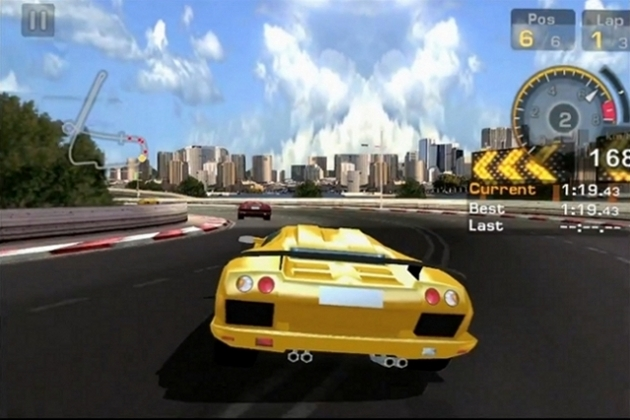
\includegraphics[width=100mm]{ge/html5_3d.jpg}
  \caption{Pierwsza gra 3D w HTML5.}
  \label{fig:html3d}
\end{figure}

Funkcjonalnością która wydaje się być szczególnie przydatna w stosunku do omawianego projektu jest możliwość rysowania kształtów geometrycznych. Przykładem wykorzystania zaprezentowano na rysunku \ref{fig:canvas1} na którym przy pomocy okręgu zaznaczono rynek główny w Krakowie i jego okolice, możliwość zmiany transparentości narysowanego kształtu pozwala aby obraz podnim był nadal widoczny.

Niestety rozwiązanie to nie może zostać wykorzystane wraz z wybranym modelem prezentacji danych geograficznych. Rysunek \ref{fig:canvas1} prezentuje potencjlne możliwośći jednak nawet analiza kodu \ref{lst:canvas} wskazuje podstawowe wymaganie wykorzystanie tego rozwiązania. Bazowy element w obrębie którego możliwa jest akcja musi być elementem typu canvas.
Otrzymany efekt jest wynikiem wykorzystania statycznego obrazu który został zaimportowany z pamięci komputera i wykorzystany jako tło. Zabieg ten pozwala na zaprezentowanie możliwości rozwiąznia ale uniemożliwia wykorzystanie funkcjonalności które dostarczane są przez Google Maps(zmiana punktu patrzenia, stopnia przybliżenia i inne). Z tego powodu zdecydowano się na zaprzestanie prac z tym konketnym rozwiązaniem i nie wykorzystanie go w docelowej aplikacji.

  \begin{figure}[H]
  \centering
    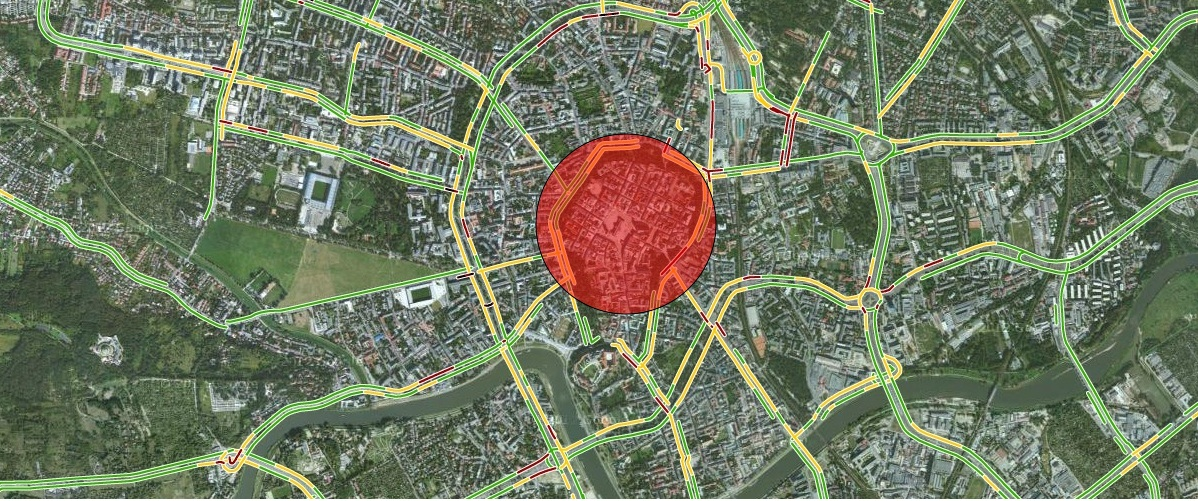
\includegraphics[width=100mm]{ge/canvas1.jpg}
  \caption{Zaznaczenie przez canvas}
  \label{fig:canvas1}
\end{figure}

\lstset{language=JavaScript}
\begin{lstlisting}[label={lst:canvas},caption={Canvas}]

      var canvas = document.getElementById('myCanvas');
      var context = canvas.getContext('2d');
      var imageObj = new Image();
	
      imageObj.onload = function() {
      context.drawImage(imageObj, 69, 50);
	  context.beginPath();
      context.arc(canvas.width / 2, canvas.height / 2, 90, 0, 2 * Math.PI, false);
      context.fillStyle = "rgba(255, 0, 0, 0.5)";
      context.fill();
      context.stroke();
      };
      imageObj.src = './gm_1.jpg';
      .
      .
      .
      <canvas id="myCanvas" width="200" height="100">
      </canvas>
\end{lstlisting}

\subsubsection{SVG}
\label{subsubsec:svg}

SVG(en. Scalable Vector Graphics) służy do prezentacji danych, tworzenia animacji i płynnych zmian kształtów. Jest to powszechnie dostępny format zapisu grafiki wektorowej który oprócz prostych kształtów geometrycznych pozwala na korzystanie z zaawansowanych filtrów i efektów.

Wykorzystywany jest wektorowy format zapisu danych, został on dokładniej omówiony w sekcji \ref{subsec:zapisWektorowy}.
W wyniku takiego zabiegu plik svg opisujący obraz graficzny może mieć mniejszy rozmiar od zapisu rastrowego, jednocześnie niezależnie od wielkości jego jakość jest taka sama.

Autorzy artykułu ``Zastosowanie języka SVG do wizualizacji danych geoprzestrzennych'' \cite{svgUse} zwracają również uwagę na tekstwoy format zapisu, jest on mniej oszczędny niż binarny ale pozwala na edycję dowolnym edytorem tekstu co pozwala na przeszukiwanie zawartości np. wyszukiwarkom internetowym.

W celach porównawczych wykorzystano logo AGH (rys. \ref{fig:aghlogo}) o rozmiarach 305x591 pikseli o gęstości 150 dpi (en. Dots per inch, określa ilość indywidualnych punktów na odcinku jednego cala, 2.54cm), po zapisie na dysku twardym zajmował on 75 KB pamięci. Następnie wykonano zapis grafiki w testowanym formacie zajmował on 3KB , efekt został przedstawiony w listingu \ref{lst:logoaghsvg}.



\begin{figure}[H]
  \centering
    
\includegraphics[width=30mm]{ge/agh_logo.jpg}
  \caption{Logo AGH}
  \label{fig:aghlogo}
\end{figure}

\lstset{language=JavaScript}
\begin{lstlisting}[label={lst:logoaghsvg},caption={Logo AGH w zapisie SVG.}]

<svg xmlns="http://www.w3.org/2000/svg" version="1.1">
<g transform="translate(0.000000,591.000000) scale(0.100000,-0.100000)" fill="#1e1e1e" stroke="none">
<path d="M984 5863 c70 -97 112 -224 143 -429 15 -97 17 -289 20 -1761 l4 -1653 99 0 100 0 0 1543 c0 933 -4 1594 -10 1673 -12 158 -37 262 -89 369 -61 127 -136 208 -265 285 l-38 23 36 -50z"/>
<path d="M1115 5878 c164 -131 256 -283 306 -503 l23 -100 3 -1627 4 -1628 94 0 95 0 0 1618 c-1 1317 -3 1631 -14 1692 -50 274 -208 455 -485 556 l-66 24 40 -32z"/>
<path  d="M1317 5867 c208 -110 326 -253 395 -477 l23 -75 3 -1647 2 -1648 100 0 100 0 0 1609 c0 1744 2 1676 -54 1826 -62 163 -173 282 -343 368 -57 29 -193 71 -263 81 -44 6 -44 5 37 -37z"/>
<path fill="#00693c" d="M52 3578 l3 -1433 23 -79 c76 -271 252 -444 522 -515 146 -38 153 -36 65 15 -170 97 -261 190 -331 339 -84 180 -78 49 -81 1668 l-3 1437 -100 0 -101 0 3 -1432z"/>
<path fill="#00693c" d="M350 3622 c0 -909 4 -1417 11 -1472 12 -101 54 -228 100 -307 73 -124 220 -238 384 -298 l70 -26 -35 27 c-61 47 -164 160 -199 218 -61 102 -100 219 -121 361 -6 44 -10 594 -10 1478 l0 1407 -100 0 -100 0 0 -1388z"/>
<path fill="#00693c" d="M650 3607 c0 -906 4 -1433 10 -1487 35 -282 148 -465 368 -594 8 -5 -3 14 -22 42 -74 103 -115 233 -141 452 -13 106 -15 346 -15 1558 l0 1432 -100 0 -100 0 0 -1403z"/>
<path fill="#a71930" d="M2237 3518 c-3 -1478 -3 -1494 -25 -1604 -27 -139 -69 -258 -121 -334 l-39 -60 40 23 c68 37 186 155 228 226 21 36 50 101 65 143 55 168 55 152 55 1686 l0 1412 -100 0 -99 0 -4 -1492z"/>
<path fill="#a71930" d="M2537 3563 c-3 -1354 -4 -1453 -21 -1523 -50 -211 -144 -362 -301 -488 l-40 -32 65 24 c255 93 402 249 472 501 l23 80 3 1443 3 1442 -101 0 -100 0 -3 -1447z"/>
<path fill="#a71930" d="M2838 3573 l-3 -1438 -23 -80 c-63 -228 -190 -384 -403 -498 -83 -44 -75 -45 56 -12 292 74 468 241 547 521 l23 79 3 1433 3 1432 -100 0 -100 0 -3 -1437z"/>
<path d="M1480 925 c-307 -69 -464 -387 -331 -670 101 -216 388 -308 704 -224 l38 10 -3 225 -3 226 -33 29 c-32 28 -35 29 -142 29 l-111 0 23 -31 c21 -29 23 -42 26 -199 l3 -169 -25 -7 c-58 -14 -155 23 -199 75 -48 58 -70 135 -71 251 -1 96 1 110 27 162 31 64 71 102 136 131 60 26 195 21 260 -11 25 -12 46 -22 48 -22 2 0 3 40 3 88 l0 89 -37 12 c-60 20 -238 23 -313 6z"/>
<path d="M244 889 c14 -17 26 -39 26 -49 0 -10 -61 -197 -135 -416 -74 -219 -135 -400 -135 -401 0 -2 38 -3 85 -3 l84 0 34 108 35 107 150 3 150 3 37 -111 37 -110 128 0 129 0 -29 83 c-97 284 -244 690 -265 732 -37 77 -58 85 -220 85 l-137 0 26 -31z m201 -369 c24 -71 41 -131 37 -134 -8 -9 -192 -7 -192 1 0 4 21 71 47 150 34 103 50 138 56 127 5 -9 28 -74 52 -144z"/>
<path d="M2263 883 c22 -37 22 -45 25 -450 l3 -413 120 0 119 0 0 190 0 190 135 0 135 0 0 -190 0 -190 120 0 120 0 0 450 0 450 -120 0 -120 0 0 -185 0 -185 -134 0 -134 0 -4 148 c-3 158 -9 176 -59 206 -20 12 -53 16 -128 16 l-100 0 22 -37z"/>
</g>
</svg>

\end{lstlisting}

\subsubsection{Google Maps Overlay}
\label{subsubsec:overlays}

Wraz z wykorzystaniem Google Maps jako bazowym źródłem danych otrzymujemy API(en.Application programming interface) umożliwiające tworzenie różnego rodzaju elementów których wygląd można w dowolny sposób edytować i zmieniać według potrzeb użytkownika.W prosty sposób możliwe jest otrzymanie efektu który został stworzony przy pomocy canvas na rysunku \ref{fig:canvas1} zachowując pełną swobodę w dalszej pracy.

Pakiet google.maps zawiera kilka klas których zadaniem jest generowanie adekwatnych obiektów. Klasy te zostały omówione poniżej.

\begin{description}
\item[Marker] \hfill \\
    Pojedyńczy punkt na mapie o określonych właściwościach które można dowolnie edytować, tak aby jego wygląd, zachowanie i położenie było zgodne z oczekiwaniami.

\item[Polyline] \hfill \\
  Linia stworzona z dwóch lub więcej punktów. Tworzone odcinki mogą być liniami prostymi lub przedstawiać zakrzywienie ziemi, nie jest możliwe tworzenie bardziej skomplikowanych łuków.

\item[Polygon] \hfill \\
  Tworzy ciąg  punktów które w określonej kolejności tworzą zamknięty obszar.

\item[Circle] \hfill \\
  Na podstawie środka i jego promienia tworzy okrąg z posiadajacy obszar wewnętrzny o określonych cechach.

\item[Rectangle] \hfill \\
  Tworzy prostokąt posiadający przeciwległe boki w określonych punktach.

\item[OverlayView] \hfill \\
  Specjalna klasa służąca do wyświetlania własnych wartswt graficznych, takich jak zewnętrzny plik graficzny. Pozwala na łatwe łączenie ogólnodostępych danych jakimi są mapy z własnymi zdjęciami, rysunkami itp.

\end{description}

Intuicyjna i szybka edycja danych jest zapewniona poprzez udostępnianie klasy "DrawingManager". Tworzy ona dodatkowy element na ekranie użytkownika służący do pracy z wartwami znajdujacymi się na ekranie. Komponent ten wymaga jedynie wybrania odpowiedniego elementu a następnie wyznaczenie wymaganych informacji,zazwyczaj są to jeden lub dwa punkty niezbędne do stworzenia elementu. Pozostałe właściwości mogą być edytowane w dalszym etapie prac według potrzeb.


\subsection{Przybliżanie zbiorów danych}
\label{subsec:aproksymacja}

Do wyznaczenia zamkniętego obszaru należy podać wszyskie punkty określające jego granice. Używając komputerów możliwy jest jedynie dyskretny zapis danych, oznacza to że tylko niektóre punkty zostają określone a odcinki pomiędzy nimi musi zostać zastąpiony danymi wygenerowanymi. Najprostrzą metodą jest połączenie poszczególnych punktów liniami prostymi otrzymując proste kształty geometryczne, przy jej pomocy posiadając 3 punkty na płaszczyźnie możliwe jest otrzymanie trójkąta. Rozwiązanie takie jest wystarczające przy tworzeniu prostych figur, posiadających małą ilość wirzchołków. Przy tworzeniu bardziej skomplikowanych staje się ono niepraktyczne, określenie setek punktów dla nieregularnego obszaru byłoby czasochłonne przez co jest nieefektywne. Rozwiązaniem tego problemu jest oszcowanie danych, określenie rozwiązania przybliżonego na podstawie znanych danych.



Można rozróżnić dwa rodzaje wyznaczanie wyniku quasi-otpymalnego:

\begin{description}
\item[Aproksymacja] \hfill \\
    Wygenerowany wynik jest przybliżeniem punktów wyjściowych, stworzona linia nie  musi przechodzić przez nie.

\item[Interpolacja] \hfill \\
    Wygenerowana funkcja iterpolacyjna przechodzi przez wszystkie punkty określony w zbiorze wejściowym, jest jego dokładnym otworzeniem. Z tego powodu nadaje się lepiej do omawianegego celu.

\end{description}


Najprostrzym rodzajem jest interpolacja funkcji sklejonych stopnia pierwszego. Określa ona zbiór prostych odcinków łączących pary poszczególnych punktów. To dzięki niej przy użyciu 3 punktów możliwe jest stworzenie trójkąta.

Interpolacja wielomianowa  polega na  określeniu jednej funkcji przechodzącej przez pożądane punkty posiadającej okeślone paramety. Złożoność tego zadania wzrasta drastycznie wraz z rozmiarem zbioru wejściowego z tego powodu nie została ona używa w omawianym przypadku.

Kolejnym z rozwiązań jest skorzystanie z krzywej Beziera. Rysunek \ref{fig:bezier} przedstawia prosty przykład pokazujący niezbędne informacje do jej stworzenia dla zbioru cztero-elementowego. Dwa punkty kontrolne, mają  za zadanie określić zachowanie ścieszki. Prosta implementacja czyni to rozwiązanie dobrym wyborem omawianego problemu.

Jego wzór dla podanego przykładu to:
\begin{eqnarray}
P(t) &= A (1-t)^{3} + 3 B t(1-t)^{2} + 3 C t^{2} (1-t) + D t^{3} \; \textrm{ dla } \; 0 \geq t \geq 1\;
\end{eqnarray}

\begin{figure}[H]
  \centering
    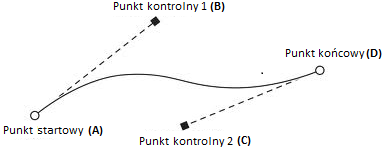
\includegraphics[width=100mm]{ge/bezier.png}
  \caption{Krzywa Beziera}
  \label{fig:bezier}
\end{figure}


\subsection{Oś czasu}
\label{subsec:os}

Tematem pracy oprócz wykorzystania i prezentacji danych na bazie informacji geograficznych jest ich połączenie z osią czasu, która pozwoliłaby na zmianę prezentowanych danych ze względu na interesujący nas okres czasu.

Ponieważ własna implementacja osi czasu która nieograniczałaby użytkownika, pozwalałaby mu w pełni korzystać  możliwości gotowej aplikacji jest zbędna w sytuacji obecności wielu tego typu rozwiązań, postanowiono wykorzystać istniejące rozwiązanie.

Przeprowadzając badania rozwiązań głównymi aspektami na które zwrócono uwagę było:


\begin{itemize}

\item

Typ licencji

Niezwykle ważne jest aby końcowy projekt był całkowicie otwarty dla dalszego rozwoju, pozwalał użytkownikom na adaptację rozwiązań dla swoich potrzeb. Z uwagi na to licencja musi pozwalać na modyfikację kodu źródłowego.

\item

Wykorzystywane technologie

Pamiętając że efektem końcowym powinien być framework odpowiadający szerokiemu gronowi odbiorców, będący jednocześnie darmowym ważne aby języki programowania wykorzystane przy jego tworzeniu też taki były. Oznacza to nie korzystanie z płatnych, wymagających licencji oprogramowań. Używane standardy powinny być rozpropagowane i używane przez szerokie grono obiorców.

\end{itemize}

Po analizie dostępnych rozwiązań zdecydowano skorzystać z widget-u o nazwie Timeline który został stworzony przej projekt SIMILE działający na uczelni MIT. Pozwala on na bardzo dużą konfigurowalność dzięki czemu jego modyfikacja, nawet bez ingerencji w kod źródłowy jest bardzo prosta.
Projekt jest w stanie stworzyć kilka pasm które będą określały interwały czasu. Pozwala to aby wynik końcowy był przejrzysty bez względu czy prezentujemy wydarzenia które miały miejsce w okresie kilku minut czy setek lat.

Rysunek \ref{fig:tm1} prezentuje przykładową oś. Pasma odpowiadają zakresom czasu, nie muszą być jednakowe w każdym miejscu. W zaprezentowanym przykładie dzień 23 listpoada uznany został za warty dokładniejszemu przyjżeniu, łatwo możemy z dokładnością co do godziny zmieniać zakres czasu.Natomiast kolejny miesiąc może być o wiele mniej ciekawy, a obszar przeznaczony dla niego być mniejszy niż ten posiadany przez wymieniony powyżej dzień.

Dla porównania \ref{fig:tm2} prezentuje o wiele prostszą konfigurację w której dolne pasmo podzielone jest przez miesiące, natomiast góre przez tygodnie.

  \begin{figure}[H]
  \centering
    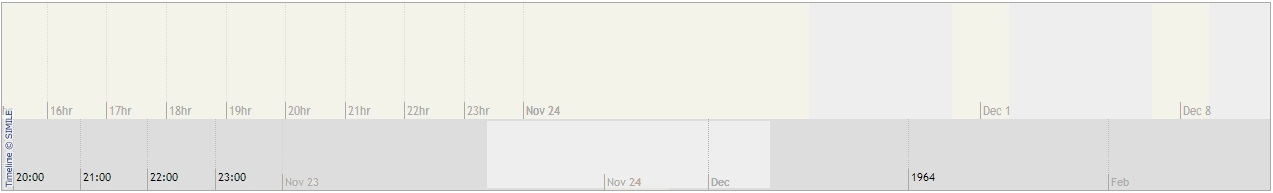
\includegraphics[width=150mm]{ge/tm1.jpg}
  \caption{Timeline}
  \label{fig:tm1}
\end{figure}

  \begin{figure}[H]
  \centering
    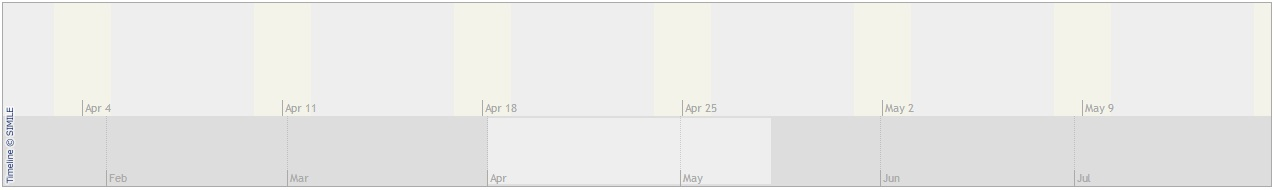
\includegraphics[width=150mm]{ge/tm2.jpg}
  \caption{Timeline - prosty przykład}
  \label{fig:tm2}
\end{figure}


\clearpage
\newpage
\section{Bezpieczeństwo danych i aplikacji}
\label{sec:bezpieczenstwo}

Tworząc aplikację która będzie używana przez dużą grupę obiorców, oprócz osób z pełnymi uprawnieniami do dowolnej akcji również osoby które nie powinny mieć możliwości zmiany danych należy przewidzieć i przygotować odpowiednie zabezpieczenia. Dostęp do dostarczanych funkcjonalności należy zapewnić poprzez zbiór ról i uprawnień, zostały one opisane w sekcji \ref{sec:uzytkownicy}.

Niezwykle ważne jest aby pamiętać o strukturze aplikacji i ograniczeniach jakie niosą za sobą wykorzystane technologie. Każdy użytkownik ``uczeń'' według nomenklatury opisanej powyżej jest w posiadaniu pliku którego edycja powinna być zachowana jedynie dla moderatora. Niestety nie jest możliwe zapewnienie nieedytowalności pliku tekstowego, z tego powodu nawet bez dostępu do uprawnień edycyjnych dostarczanych przez framework każdy może edytować plik w edytorze tektsowym, zmienić granice obszarów czy chociażby przedziały czasowe. Aby użytkownicy mieli pewność że plik z którego korzystają i mapa stworzona na jego podstawie jest wiarygodna i posiada poprawne dane proponowanym rozwiązaniem jest wykorzystanie jednego z algorytmu tworzących skrót z dowolnego ciągu danych, jednym z najczęściej wykorzystanym do takich celów jest MD5. Otrzymany wynik można zamieścić na serwerze w widoczny miejscu obok pliku z danymi w miejscu gdzie jedynie moderator ma dostęp. Dzięki takiej operacji użytkownik będzie mógł porównać wygenerowany skrót pliku którego chce użyć z wartością na stronie, identyczne wartości potwierdzą autentyczność danych.

\subsection{Funkcje haszujące}
\label{sec:hashfunction}

W pewnych sytuacjach nie potrzebujemy lub nie chcemy przechowywać oryginalnego pliku lub ciągu znaków. Częstym wykorzystaniem jest utworzenie skrótu hasła w module logowania do różnych aplikacji. Czynność ta utrudnia poznanie rzeczywistych wartości w momencie dostępu do nich przez nieuprawnione osoby. Jedną z cech dobrej funkcji haszującej jest
spełnienie wymagań dla funkcji jednokierunkowej. Wymagane jest aby funkcja była łatwa do obliczenia ale trudna, lub wręcz niemożliwa do odwrócenia.

Innym częstym wykorzystaniem, zaproponowanym w poprzedniej sekcji, jest weryfikacja integralności pliku lub wiadomości. Umieszczenie w jedym miejscu pliku i jego skrótu umożliwia sprawdzenie czy plik który posiadamy jest identyczny z tym znajdującym się na stronie, w przypadku braku zgodności możliwe jest ściągnięci poprawnej wersji, w pozostałych sytuacjach posiadamy pewność autentyczności danych bez potrzeby każdorazowego ściągania pliku z serwera, oszczędzamy przez to czas poświęcony na ściągnięcie pliku, który może zajmować wiele megabajtów.

Istnieje wiele funkcji haszujących, wybór konkretnej z nich zależy od celu użycia najpopularniejszymy są MD5 i SHA-1.

\begin{itemize}
\item
MD5

Opracowany w 1991 roku przez Rona Rivesta, z dowolnego ciągu danych generuje 128-bitowy sktót, pozwala to na utworzenie 32 znakowego ciągu w systemie szesnastkwoym. Ważną cechą jest zmiana skróty w przypadku najmniejszej edycji wejściowych danych. Tabela \ref{tab:hashresult},stowrzona przy pomocy strony \underline{\texttt{http://www.sha1-online.com/}}, prezentuje przykład zmiany jednej litery, zmiany ``ó'' na ``o'' w słowie Kraków. Wygenerowany skrót dla tej wartości jest zupełnie inny.Z uwagi na szybkość działania jest powszechnie używana.

\item
SHA-1

Przedstawiciel funckji z rodziny SHA, opublikowany w 1995 roku. W przeciwieństie do MD5 przy zapisie skrótu korzysta z 160-bitów, oznacza do 40 znaków w systemie heksadecymalnym.

\item
SHA-2

Zbiór czterech wariantów zastępujących SHA-1. Wersją zapewniającą najwyższą obecnie niezawodność i bezpieczeństwo jest SHA-512, do zapisu wykorzystuje 512 bitów co pozwala na otrzymanie 128 znakowego skrótu.

\end{itemize}

\begin{table}[H]
    \centering
    \begin{tabular}{|l|l|l|}
    \hline
    Algytm & Wejściowy ciąg & Wygenerowany skrót  \\ \hline
    MD5 & AGH Kraków &    c9c16a90d4938da799b5aa7d6f37edce  \\ \hline
    MD5 & AGH Krakow &    fc6a83206673002588490eb05b89313f  \\ \hline
    SHA-1 & AGH Kraków &  6205880f638b3e584578125b14231c30c3ab9fea  \\ \hline
    SHA-1 & AGH Krakow  & a536aa59ed829801cd0f099c4ae3ba34ca57ca9f \\ \hline
    SHA-512 & AGH Kraków &  49d9e2deb053a58dcb0a778758e5(...)61499145e36353  \\ \hline
    SHA-512 & AGH Krakow  & 6b65c56ca2e5567a5f18dd0d7465(...)f46166c29d7105 \\ \hline
    \end{tabular}
    \caption{Rezulaty funkcji haszujących}
    \label{tab:hashresult}
\end{table}


\clearpage
\newpage
\section{Optymalizacja rozwiązania}
\label{sec:optymalizacja}
 

\subsection{Wydajność parsera}
\label{subsec:wydajnosc}

W celach sprawdzenia wydajności zaimplementowanego parsera przeprowadzono testy porównawcze. W pierwszej próbie wykorzystano dwa pliki zawierające dane w formacie który pozwolił na jego analizę, pierwszy ``plik1.kml''  składał się z jednego obszaru i jednego stylu określającego preferencje graficzne, jego dokładana zawartość została zawarta w załączniku \ref{sec:akml}. Drugi plik ``plik2.kml'' zawierał informacje o granicy wszystkich stanów USA, na potrzeby badań on również zawierał informacje o jednym stylu.
Wykonano proces wczytania ich zawartości, mierząc za każdym razem czas potrzebny na zakończenie procesu. Wyniki zamieszczono w zbiorczej tabeli \ref{tab:speedTest}.

Dokładne informacje dotyczące zawartości plików zamieszczono w tabeli \ref{tab:testFile}

\begin{table}[H]
    \centering
    \begin{tabular}{|l|l|l|}
    \hline
    Nazwa pliku & Ilość punktów & Ilość poligonów \\ \hline
    plik1.kml & 13 & 1 \\ \hline
    plik2.kml & 13697 & 133 \\ \hline

    \end{tabular}
    \caption{Pliki testowe}
    \label{tab:testFile}
\end{table}


\begin{table} [H]
    \centering
    \begin{tabular}{|l|l|l|}
    \hline
    Test & 13 punktów & 12697 punktów \\\hline
    I & 3 & 343 \\\hline
    II & 13 & 449 \\\hline

    \end{tabular}
    \caption{Czas dostępu [ms]}
    \label{tab:speedTest}
\end{table}

\subsection{Reprezentacja graficzna}
\label{subsec:showing}

W celu optymalizacji działania aplikacji zastosowano kilka rozwiązań mających na celu przyścieszenie działania. Dotyczą one sposobu w jaki aplikacja renderuje graficzna częśc projektu.


\begin{description}
\item[Stopniowa generacja obiektów]\hfill \\
Nie wszystkie obiekty dotyczące mapy są renderowane podczas jej inicjalizacji. Wstępna konfiguracja pozwala na stworzenie mapy z osią czasu nie pokazującą całego przedziału czasowego do którego odwołują się informacje wejściowe, możliwe jest ustawienie aby na ekranie pojawiły się informacje dotyczące wydarzeń z jednoego dnia podczas gdy dane mogą zawierać informacje z okresu kilku lat. Stworzony algorytm można przedstwić w najstępujących krokach.

\begin{enumerate}
\item
Renderowanie jedynie elementów widocznych na ekranie (mających miejsce w widocznym okresie czasu).

\item
Renderowanie dodatkowych elementów zawierających się w otoczeniu wynoszącym 10\% aktualnego okresu a następnie ukrycie ich. Takie rozwiązanie pozwala, w większości przypadków, na rederowanie nawet dużych i skomplikowanych obiektów bez wpływu na działanie użytkownika(posiada on dane wygenerowane w pkt. 1 i nie oczekuje na wygenerowanie kolejnych).

\item
Podczas przesunięcia lini czasu w pierwszym momencie elementom w najbliższym sąsiedztwie ustawiana jest flaga widoczności, jeśli zmiana okresu była niewielka akcja ta jest wystarczająca aby pokazać wszystkie wyamgane elementy, w przeciwnym przypadku nastepuje generacja brakujacych. W obu przypadkach po zakończniu powtarzay jest pkt 2. Obiekty które nie powinny być widoczne nie są niszczone jedynie chowane.

\end{enumerate}

\item[różne poziomy test]\hfill \\

\end{description}

\chapter{Opis rozwiązania}
\label{cha:Opis rozwiązania}

W poniższym rozdziale omówione zostaną kroki pracy.

\section{Transmisja danych}
\label{sec:transmisjaDanych}

Pierwszym aspektem który należy rozwiązać jest sposób przesyłania danych. Problem ten jest szczególnie istotny w omawianej pracy z uwagi na możliwość przesyłania informacji o granica lub innych liniach przezentowanych na mapie. Do opisu kwadratowego obszaru wymagane jest przesłanie informacji o 4 punktach. Jeżeli będziemy chcieli przekazać dokłądniejszy zarys obszaru, zaprezentować granicę państwa lub linię frotnu wojennego linia prosta w większości przypadków będzie zbyt ogólnym przybliżeniem, nie oddającym prawdziwej sytuacji.

Z raportu Akamai wynika że śrenia przepływność łączy internetowych dla użytkowników korzystających z puli adresów IP przeznaczonych dla Polski w I kwartale 2012 r. wynosiła 5Mb/s  \underline{\texttt{http://www.rp.pl/artykul/924483.html}} (dostęp 13.04.2014). Jest to bardzo dobry wynik któy plasuje Polskę w czołówce rankingu. Pomimo tego nie można pominąć faktu optymalizacji zapytać i danych przesyłanych, wymieniane dane pomiędzy użytkownikiem a serwerem powinny być jak najmniejsze. Duża popularność urządzeń mobilnych w których dostęp do internetu jest zapewniany często poprzez sieć bezprzewodową a dostęp do interentu nie jest jeszcze tak dogodny jak jest to w przypadku użytkowników stacjonarnych  wymusza optymalizację.

Kolejnym powodem dla którego odpowiedzi serwera powinny być jak najlżesze jest koszt pracy samego serwera. Jest to szczególnie widoczne w dużych aplikacjach mających wiele urzytkowników, czas jaki jest przeznaczany dla pojedyńczego użytkownika jest mnożony przez ich ilość. Z tego powodu zawsze podczas zwiększania ilości użtkowników korzystających z aplikacji następuje czas w którym należy zacząć korzystać z dodatkowego serwera. Celem programisty tworzącego kod który będzie wykorzystywał zasoby serwera(zarówno czas jak i pamięć) jest dbanie aby moment w którym niezbędne będzie korzystanie z większej ilośći maszym nastąpił przy jak największej ilości użytkowników.

xml - 729  557
json - 695  400


\section{Możliwości HTML5}
\label{sec:html5}

HyperText Markup Language,  hipertekstowy język znaczników
Pozwala na opisanie struktury informacji zawartych na stronie internetowej, to dzięki niemu przeglądarka moze rozróżnić takie elementy jak hiperłącze,akapit czy chociażby nagłówek.

Podobnie jak w przypadku XML, tak i tutaj wymagane jest aby wykorzystywane znaczniki umieszczane były w nawiasach ostrokątnych, a każdy z nich miał swoje domknięcie.

Poprawnym zapisem jest <p>Wiadomość<p> który oznacza pojedyńczy akapit. Zapis <p>Wiadomość<p>, który różni się od poprzedniego brakiem znaku "" w drugim znaczniku, czyni to ten zapis niepoprawnym. Istnieje możliwość aby wykorzystać pojedyńczy znacznik przykładem jest <br> określający nową linię która będzie widoczna na stronie.

Obecnie używany standart HTML4 ma niestety wiele ograniczeń, z tego powodu pracowano nad jego następnikiem. 22 stycznia 2008 W3C opublikował HTML5, wtedy jeszcze jako jedynie szkic.

Bardzo ciekawym i wartym zainteresowania dodanym elementem w nowej wersji jest obecność znaczniku canvas. Pozwala on na dynamiczne , skryptowe renderowanie kształtów i obrazów. Dzięki temu obiektowi możliwe stało się tworzenie animacji czy nawet gier działających w przeglądarce bez konieczności używania dodatkowych wtyczek czy programów.

\underline{\texttt{http://techtrendy.pl/title,Pierwsza-gra-3D-napisana-w-HTML5,wid,14102779,wiadomosc.html?ticaid=6107dc}}

Przykładem wielkich możliwości jakie dostarcza udoskonalony język jest fakt iż już w roku 2011 powstała pierwsza trójwymiarowa gra stworzona w całości przy użyciu HTML5. Przykład grafiki widoczny jest na rysunku \ref{fig:html3d}.
Wcześniej takie efekty możliwe były jednynie przy wykorzystaniu technologi Flash, jej wadą była drudność edycji gotowego produktu, wyganało to specjalnego oprogramowania. Fakt tworzenia pliku wykonywalnego którego nie było możliwości edycji wymuszał dostęp do kodów źródłowych, czyli plików które tworzył autor programu.

\begin{figure}[H]
  \centering
    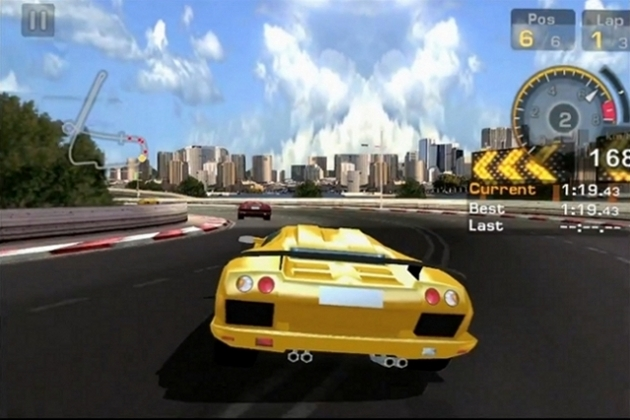
\includegraphics[width=100mm]{ge/html5_3d.jpg}
  \caption{Pierwsza gra 3D w html5.}
  \label{fig:html3d}
\end{figure}

Konkretną funkcjonalnością która wydaje się być przydatna w omawianym projekcie jest możliwość rysowania kształtów geomeycznych, również na innych obrazach. Przykładem wykorzystania tej technologi jest \ref{fig:canvas1} na którym przy pomocy okręgu zaznaczono rynek główny w Krakowie i jego okolice, możliwość zmiany przejżystości narysowanego kształtu pozwala aby obraz podnim był nadal widoczny.

  \begin{figure}[H]
  \centering
    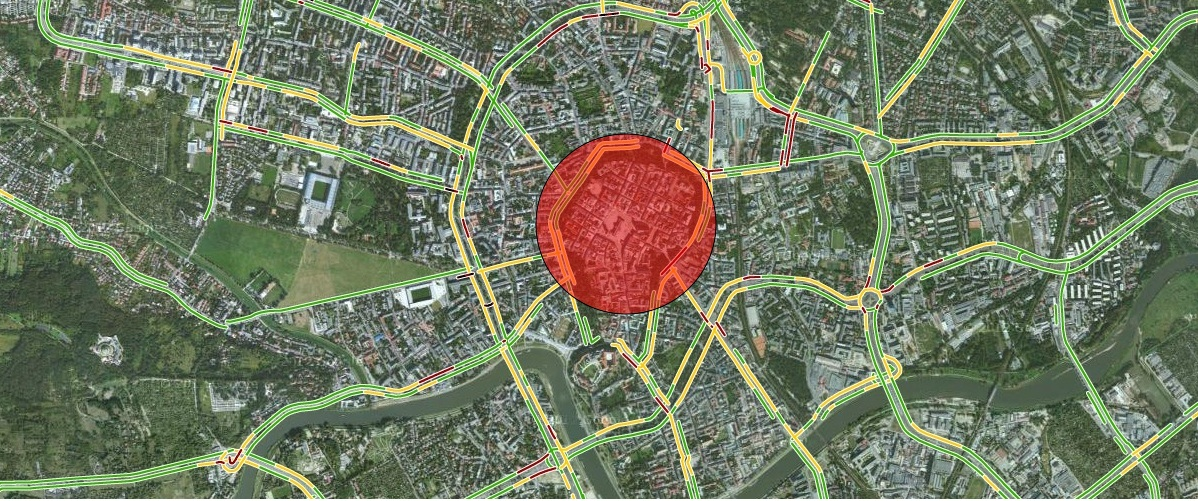
\includegraphics[width=100mm]{ge/canvas1.jpg}
  \caption{P.}
  \label{fig:canvas1}
\end{figure}

\lstset{language=JavaScript}
\begin{lstlisting}[caption=json]

      var canvas = document.getElementById('myCanvas');
      var context = canvas.getContext('2d');
      var imageObj = new Image();
	
      imageObj.onload = function() {
      context.drawImage(imageObj, 69, 50);
	  context.beginPath();
      context.arc(canvas.width / 2, canvas.height / 2, 90, 0, 2 * Math.PI, false);
      context.fillStyle = "rgba(255, 0, 0, 0.5)";
      context.fill();
      context.stroke();
      };
      imageObj.src = './gm_1.jpg';

\end{lstlisting}

\subsection{Wykorzystanie HTML5}
\label{subsec:htmluse}

Wstępne założenia zakładały wykorzystanie możliwości rysowania kształtów przy użyciu ogólnodostępnych map. Rozważania w sekcji \ref{sec:Rodzaje map} wskazały że najlepszym wyborem są Google Maps. Niestety opcja rysowania kształtów któa dostarcza HTML5 wymaga uzycia znacznika canvas, nie jest to kompatybilne z metodą wykorzystywania maps dostarczanych od omawianej firmy która wymaga wykorzystanie znacznika div.W momencie tworzenia tej pracy nie ma możliwości współpracy wybranych map z technologią rysowania kształtów geometrycznych. Sytuacja taka wymusza wykorzystanie innego rozwiązania do tworzenia interesujących nas warstw.

\subsection{Storage}
\label{subsec:storage5}
Inną ciekawą funkcją omówioną w podręczniku do HTML5  \cite{html5dive} jest Storage. Pozwala on na przechowywanie danych w przeglądarce użytkownika. Różnicą w stosunku do ciasteczek które również potrafią przechowywać informacje o konretnym użytkonwniku jest:
\begin{itemize}
\item
Większy rozmiar dostępnej pamięci m.in. Chrome 5MB \nocite{chrome5mb}, IE 10
\item
Informacje przechowywane są po stronie użytkownka, nie są przesyłane za każdym razem do serwera.
\item
Informacja może być przechowywana przez długi okres czasu.
\end{itemize}



Dodatkowo nie można pominąć faktu istnienia dwóch rodzaii tej pamięci.
\begin{itemize}

\item
Session Storage
Dane przechowywane są w kontekście sesji użytkownika, są one tracone w momencie zamknięcia okna przeglądarki.

\item
Local Storage
Teoretycznie dane są przechowywane w nieskończoność, do momentu kiedy użytkonwik nie usunie ich. Zamknięcię sesji nie powoduje czyszczenia danych.

\end{itemize}

Powodem który wymaga wykorzystania tego typu pamięci jest możliwość przechwowywania danych nad którymi użytkonwik pracuje w aktualnym czasie. Nie potrzebuje on informacji które były dla niego istotne podczas poprzedniej wizyty,sesji. Sytuacja ta jednoznacznie wskazuje że lepszym wyborem jest wybór pamięci sesyjnej(Session Storage).


Wadą tej pamięci jest jej interfejs. Obecnie przechowywany sposób danych to mapowanie w postaci napis->napis. Wymusza to aby każde dane które chcemy przechować muszą być w formie ciągu znaków. Przykład \ref{lis:storage} przedstawia w jaki sposób możemy obiekt zawierający imię i nazwisko zapisać w pamięci. Linia 4 przedstawia obiekt w postaci któej chcielibyśmy go przechować. Niestety zwykłe przypisanie do zmiennej w pamięci powoduje że jedynie typ instancji zostaje zapisany. Aby móc zapisać w poprawnej formie dane musimy doknać serializacji danych. Czynność tą możemy wykonać przy pomocy metody stringify z obiektu JSON, wynikiem jest ciąg znaków który możemy bez problemu zapisać w pamięci sesyjnej. Do odzyskania pierwotnego obiektu, odtworzenia go z zapisanego napisu wykorzystujemy metodę parse również z obiektu JSON.

\lstset{language=JavaScript}
\label{lis:storage}
\begin{lstlisting}[caption=json]
      uzytkownik={};
      uzytkonwik.imie='Jan'
      uzytkownik.nazwisko='Kowalski'
      //uzytkownik : Object {imie: "Jan", nazwisko: "Kowalski"}
      
      sessionStorage.u1 = uzytkownik
      //sessionStorage.u1 : "[object Object]"
      
      sessionStorage.u2 = JSON.stringify(uzytkownik)
      //sessionStorage.u2 : "{"imie":"Jan","nazwisko":"Kowalski"}"
      
      uzytkonwik2 = JSON.parse(sessionStorage.u2)
      //uzytkonwik2 : Object {imie: "Jan", nazwisko: "Kowalski"}
\end{lstlisting}



Wsparcie dla pamięci Storage nie jest obecne zazwyczaj w nowszych wersach przeglądarek. Na stronie \underline{\texttt{http://www.html5rocks.com/en/features/storage}} możemy sprawdzić aktualny stan większości przęglądarek.

\subsection{Web SQL Database}
\label{subsec:websql}

Koljenym ciekawym rozwiązaniem problemu przechowywania danych po stronie klienta jest Web Sql Database. 
Jest to baza danych która została umieszczona po stronie klienta. Jest to dodatkowa warstwa która korzysta z SQlite.
Zaletą takiego rozwiązania jest przeżucenie kosztów obliczeniowych na stronę klienta,operacje takie jak sortowanie, filtrowanie na bazie danych wykonywane są przy wykorzystaniu zasobów komuptera klienta.

Nie wątpliwą zaletą w stosunku do omówionej w rozdziale \ref{subsec:storage5} pamięci jest możliwość ustalenia wielkości zalokowanej wielkości pamięci. Dzięki temu nie jesteśmy ograniczenie granicą maksymalnie 5MB w więkoszości przeglądarek. 

Przykład wykorzystania został zaprezentowany na przykładzie. Po stworzeniu bazy danych o nazwie ExampleDataBase i rozmiarze 2MB możemy korzystać z niej jak z każdej innej bazy danych. Możliwe są m.in. operacje tworzenia table(linie 3-5), wstawiania danych(parametry podajemy po treści zapytania, następnie możemy podać funkcje które zostaną wykonane w momencie sukcesu lub w przypadku wystąpienia błędu). Odczyt danych (linie 13-18) jest analogiczny do pozostałych operacji, dodatkowo pokazano w jaki sposób możliwa jest iteracja po otrzymanych wynikach.

Wadą tego rozwiązania jest jego popularność.Na stronie browser stats  możemy sprawdzić jaka jest aktualnie popularność poszczególnych przeglądarek na świecie. Porównując te dane z dostępnością Web Sql dostępną na stronie \underline{\texttt{http://www.html5rocks.com/en/features/storage}} (dostęp) możemy wnioskować że prawie 45\% użytkowników( korzystających z IE i Firefox) nie mogą korzystać z tego rozwiązania. Fakt ten dyskfalfikuje je.

\lstset{language=JavaScript}
\label{lis:webSql}
\begin{lstlisting}[caption=json]
      var db = window.openDatabase("ExampleDataBase", "1.0", "Description", 2 * 1024 * 1024);
      
      db.transaction(function(tx) {
        tx.executeSql("CREATE TABLE TableTest (id REAL UNIQUE, text TEXT)");
      });
      
      db.transaction(function(tx) {
        tx.executeSql("INSERT INTO TableTest (id, text) VALUES (?, ?)", [1, 'test'],
        onSuccess,
        onError);
                });
                
      db.transaction(function(tx) {
        tx.executeSql("SELECT * FROM TableTest", [], function(tx, result) {
            for (var i = 0, item = null; i < result.rows.length; i++) {
                ...
			}
        });
      });
\end{lstlisting}

\subsection{IndexedDB}
\label{subsec:indexDB}

Trzecim rozwiązaniem jest indexDb.

\section{Oś czasu}
\label{sec:timeLine}

Tematem pracy oprócz wykorzystania i prezentacji danych na bazie informacji geograficznych jest ich połączenie z osią czasu, która pozwoliłaby na zmianę prezentowanych danych ze względu na interesujący nas okres czasu.

Ponieważ własna implementacja osi czasu która nieograniczałaby użytkownika, pozwala mu w pełni korzystać z możliwości pełnej aplikacji, która tylko w części składa się z możliwości manipulacji czasem postanowiono wykorzystać istniejące rozwiązanie.

Przeprowadzając badania rozwiązań głównymi aspektami na które zwrócono uwagę było:

\begin{itemize}

\item

Typ licencji
Niezwykle ważne jest aby końcowy projekt był całkowicie otwarty dla dalszego rozwoju, pozwalał użytkownikom na adaptację rozwiązań dla swoich potrzeb. Z uwagi na to licencja musi pozwalać na nieograniczoną modyfikację kodu źródłowego.

\item

Wykorzystywane technologie
Pamiętając że efektem końcowym powinien być framework odpowiadający szerokiemu gronowi odbiorców, będący jednocześnie darmowym ważne aby języki programowania wykorzystane przy jego tworzeniu też taki były. Oznacza to nie korzystanie z płatnych, wymagających licencji oprogramowań. Używane standarty powinny być rozpropagowane i używane przez szerokie grono obiorców.

\end{itemize}

Po długich i wnikliwych poszukiwaniach zdecydowano skorzystać z widget-u o nazwie Timeline który został stworzony przej projekt SIMILE działający na uczelni MIT. Pozwala on na bardzo dużą konfigurowalność dzięki czemu jego modyfikacja, nawet bez ingerencji w kod źródłowy jest bardzo prosta.
Projekt jest w stanie stworzyć kilka pasm któe będą określały interwały czasu. Pozwala to aby wynik końcowy był przejżysty bez względu czy prezentujemy wydarzenia które miały miejsce w okresie kilku minut czy setek lat.

Problemem który pojawił się było połączenie wybranego sposobu prezentacji osi czasu z mapą i elementami które powinny zmieniać się wraz z upływem czasu.

Rysunek \ref{fig:tm1} prezentuje możliwości tego projektu. Pasmo odpowiadają zakresom czasu, nie muszą on jednak być jednakowe w każdym miejscu. W zaprezentowanym przykładie dzień 23 listpoada uznany został za warty dokładniejszemu przyjżeniu,łatwo możemy z dokładnością co do godziny zmieniać zakres czasu.Natomiast kolejny miesiąc może być o wiele mniej ciekawy, a obszar przeznaczony dla niego być mniejszy niż ten posiadany przez wymieniony powyżej dzień.

Dla porównania \ref{fig:tm2} prezentuje o wiele prostszą konfigurację w której dolne pasmo podzielone jest przez miesiące, natomiast góre przez tygodnie.

  \begin{figure}[H]
  \centering
    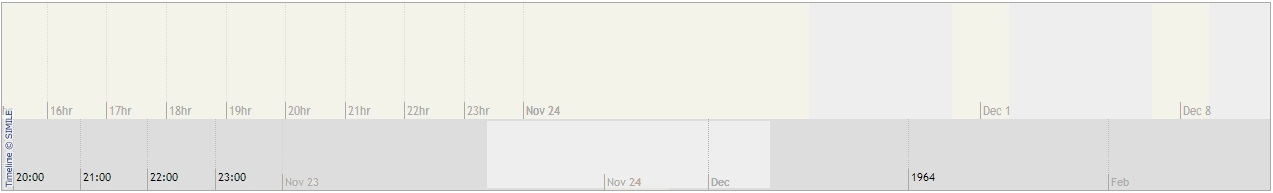
\includegraphics[width=150mm]{ge/tm1.jpg}
  \caption{Timeline}
  \label{fig:tm1}
\end{figure}

  \begin{figure}[H]
  \centering
    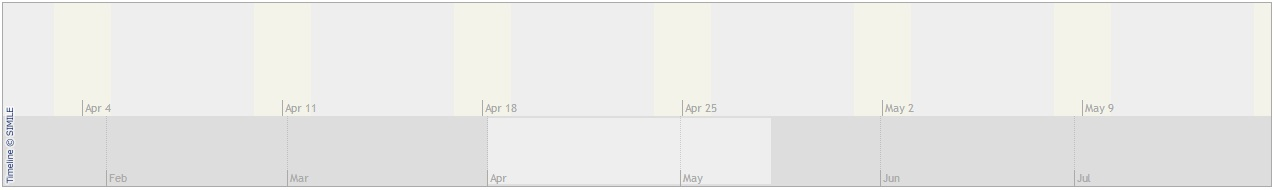
\includegraphics[width=150mm]{ge/tm2.jpg}
  \caption{Timeline 2}
  \label{fig:tm2}
\end{figure}
\section{Przybliżanie wyników}
\label{sec:przyblizanie}

Zmniejszanie ilości makretów w zależności od stopnia przyblizenia


\section{Parser kml}
\label{sec:scaner}



Format KML jest używany do reprezentacji danych graficznych w aplikacjach firmy Google, takich jak Google Maps czy Google Earth. Oparty jest na standardzie XML, wrażliwy na wielkość liter, wymusza ścisłą poprawność danych z formatem. Oznacza to że każdy tag, element ma ścisle określone miejsce i nie może pojawić się nigdzie indziej.


Aby tworzona aplikacja miała możliwość współpracy ze stworzonymi wczesniej zbiorami danych, mapami mimo faktu iż informacje te nie będą w pełni wykorzystywały możliwości frameworku, stworzony został parser plików kml. Dzięki temu możliwy jest import danych, uzupełnienie ich o dodatkowe informacje i zapis do własnego formatu.






\section{Interferjs}
\label{sec:Interferjs}




\chapter{Implementacja}
\label{cha:implementacja}

W działaniu programu można wyodrębnić 2 główne etapy, jest to dostarczenie danych zgonych formatem aplikacji a następnie ich wyświetlenie. Zapewniono obsługę zewnętrznych plików, zarówno zapisanych w standardzie KML jak i jego rozszeżenia stworzonego na potrzeby projektu. Interpretacja graficzna danych została zoptymalizowana na potrzeby pracy z dużymi zbiorami danych, tak aby wyświetlenie nawet dużej ilości informacji umożliwiało dalszą pracę.


\section{Struktura projektu}
\label{sec:structure}

Struktura klas w aplikacji została stworzona w oparciu o wzorzec projektowy MVC(en. Model–view–controller). Zakłada on podział na 3 główne warstwy, są nimi:

\begin{itemize}
\item
Controller - jego zadaniem jest przyjmowanie danych wejściowych i na ich podstawie odpowiednia reakcja, która może być aktualizają modelu lub warstwy prezentacyjenj.  W aplikacji funkcję tą spełniają servisy i kontrolery.
\item
View - warstwa prezentacyjna, zapewnia wizualiną prezentację infrmacji. Rolę tą w omwianym projekcie spełnia HTML i CSS.
\item
Model - przechowuje dane, stanowi bazę danych. Jego rola została przeniesiona na natywne rozwiązanie jakim jest Storage.
\end{itemize}

Założenia wzorca nie zostały w pełni spełnione, jego adaptacja została wykonana na potrzeby omawianego projektu. Stworzono podstawy do rozwoju i prostej adaptacji rozwiązania do potrzeb konkretnego klienta, w bardzo prosty sposób można zmienić między innymi sposób przechowywania danych aby spełnić wymagania klienta.


Zastosowano również paradygmat odwrócenego sterowania(en. Inversion of control,IoC) polegający na przeniesieniu poza obiekt metod służących do kontroli jego poszczególnych elementów. Główną zaletą tego podejścia jest uproszczona kongiguracja programu do potrzeb użytkownika. Przykładem zastosowania jest metoda korzystania z filtrów w aplikacji, które mogą być tworzone przez użytkownika. Ich potencjalnie duża ilość wczytywana jednocześnie podczas startu generowałaby zbędne obciążenie, obecnie są one pomijane podczas inicjacji i wczytywane pojedyńczo jedynie wtedy gdy ich obecność jest niezbędna.


Struktura klas obecnych w aplikacji została zaperzentowana na rysunku \ref{fig:classDiagram2}.

\begin{center}
\begin{figure}[H]
\centering
     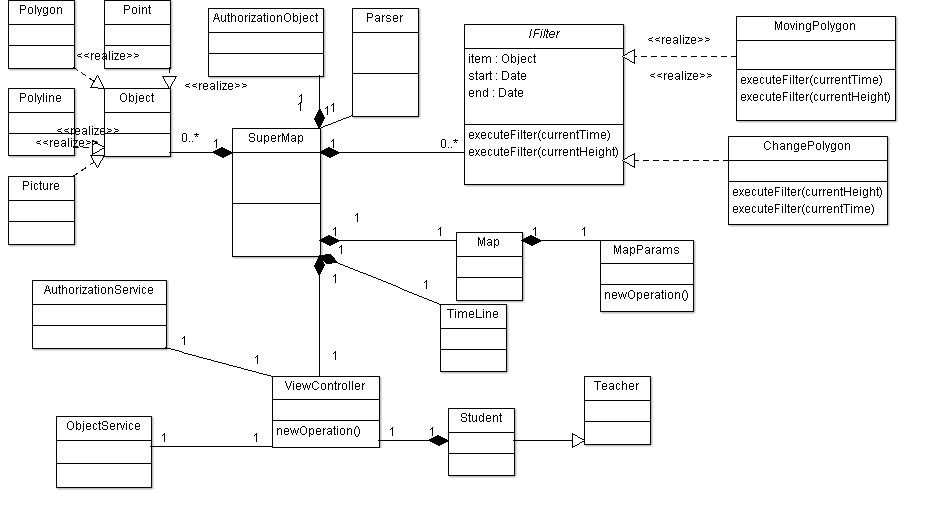
\includegraphics[angle=270,origin=c,width=130mm]{ge/smieci/ClassDiagram.png}
      \caption{Diagram klas.}
       \label{fig:classDiagram2}
\end{figure}
\end{center}

\section{Minimalna konfiguracja}
\label{sec:minimum}

Do rozpoczęcia korzystania z gotowej aplikacji należy zapewnić obecność konfiguracji niezbędnej do jej konfiguracji na docelowej stronie. Przykład minimalnej wersji która spełnia wymagane został pokazany w listinu \ref{lst:minconf}.

Z uwagi na naturę projektu, aplikacja wykorzystywana w przeglądarce, jak każdy dokument stworzony w HTML musi składać się z 3 głównych części:


-lini zawierającej informację o używanej wersji HTML, w poniższym przykładzie dotyczy ona HTML5

-deklaracji sekcji header, zawiera odwołania do zewnętrzych plików i delkaracje funcji, styli

-część właściwa strony która zawiera infromacje właściwe, widoczne dla użytkownika storny.

Linie 5-7 mają za zadanie wczytanie zewnętrzych plików zawierające delkaracje metod w JS. 8 wczytuje plik zawierający główną klasę frameworku, poniżej znajduje się wczytanie niezbędnych styli CSS dla działąnia osi czasu. 13-23 jest to opis metody która inicjuje działanie mapy, jest ona wykonywana po załadowaniu statycznych fragmentów strony.

\lstset{language=JavaScript}
\begin{lstlisting}[label={lst:minconf},caption={Minimalna konfiguracja.}]

<!DOCTYPE html>
<html>
  <head>
    <script type="text/javascript" src="https://maps.googleapis.com/maps/api/js?sensor=false&key={KEY_ID}">
    <script type="text/javascript" src="./js/specialMap/lib/jquery-1.6.2.min.js"></script>
    <script type="text/javascript" src="./js/specialMap/lib/mxn/mxn.js?(googlev3)"></script>
    <script type="text/javascript" src="./js/specialMap/lib/timeline-1.2.js"></script>
    <script type="text/javascript" src="./js/specialMap/src/timemap.js"></script>
    <script type="text/javascript" src="./js/specialMap/src/utils.js"></script>

    <link type="text/css" rel="stylesheet" href="./css/examples.css"/>

    <script>
    var sm;
    $(function() {
        tm = SpecialMap.init({
            mapDivId: "mapId",
            timeDivId: "timeId",
            dataType: "sessionStorage",
            bandIntervals: [
	            Timeline.DateTime.YEAR
	        ],
        });
    });
  </head>
  <body>
        <div id="specialMap">
            <div id="timeId"></div>
            <div id="mapId"></div>
        </div>
  </body>
</html>
\end{lstlisting}/


\section{Interfers do map}
\label{sec:mxn}

W procesie badań literaturowych podjęto decyzję aby jako głównego źródła map wykorzystać Google Maps \ref{subsec:Rodzaje map}.Postanowiono jednocześnie umożliwić użytkownikowi możliwość zmiany i wyboru innego dostarczyciela danych. Niestety nawet krótka analiza interfejsów dostarczaych do pracy nad różnymi typami map wskazuje na brak kompatybilności pomiędzy nimi, oznacza to brak możliwości stworzenia jednej implementacji działąjącej na różnych typach. Problem ten rozwiazano potrzez wykorzystanie Mapstraction, biblioteki której zadaniem jest płynne przechodzenie pomiędzy różnymi dostarczycielami i ich interfejsami.

Listening \ref{lst:mapstraction} pokazuję przykład wykorzystania biblioteki. Stworzenie instancji Mapstraction polega na wywołaniu konstruktora z podaniem id elementu który znajduje się na stronie i będzie używany jako nasza mapa a także typ mapy. Rezultatem jest obiekt kóry posiada wspólny interjeft dla różnych dostarzcycieli danych.

\lstset{language=JavaScript}
\begin{lstlisting}[label={lst:mapstraction},caption={Wykorzystanie Mapstraction.}]

var map = new Mapstraction(mapId, 'google');

var point = new mxn.LatLonPoint(0,0);
var marker = new mxn.Marker(point);
map.addMarker(marker);

\end{lstlisting}/



\section{Odczyt danych}
\label{sec:idata}

Tak jak zostało omówione w sekcji \ref{sec:dataformat} do przechowywania danych stworzono format rozszeżający istniejący obecnie KML.Takie podejście pozwala na swobodne tworzenie i edycję plików wejsciowych, brak ograniczeń. Jednocześnie zachowując minimalną strukturę obecnie istniejącego formatu pozwala na dostęp od dużej bazy istniejących informacji.

W celu odczytu i konwersji danych z pliku zapisu ich w pamięci sesyjnech przęglądarki omówionej w rozdziale \ref{subsec:storage5} stworzona została klasa FileParser. Posiada ona jednoargumentowy konstruktor przyjmujący ciąg znakowy będący zawartośćią pliku .

Ze względów bezpieczeństwa JavaScript nie zezwala na bezpośredni dostęp do plików lokalnych uzytkownika. Jest to pozytywne zachowanie zapewniające że żaden kod nie jest w stanie bezwiednie zmieniać zawartość dysku.

Wymusza to korzystanie z event-ów które będą aktywowane w momecie kiedy plik zostanie wybrany. W momencie zakończenia procesu odczytu zawartość pliku przekazywana jest do parsera który zapisuje dane w pamięci przeglądarki.

W przeciwieństwie do języków które posiadają klasyczną koncepcję klasy JavaScript posiada jedynie obiekt, z uwagi na ten fakt tworzenie metod i procedur następuje odmiennie. Istnieją 3 podstawowe sposby:

\begin{itemize}
\item
Wykorzystanie globalnej funkcji. Tworzony obiekt zawiera odowłanie do ciała metody, które jest globalne. Wadą takiego rozwiązania jest tworzenie wielu globalnym funkcji których nazwa może kolidować z nazwazmi w wykorzystywanych bibliotekach.
\item
Stworzenie funkcji wewnętrzej. Podobnie jak w poprzednim przypadku tworzona jest funkcja , tym razem jej ciało znajduje się w obiekcie. Minusem jest konieczność odtwarzania metody przy każdej sytuacji tworzenia obiektu. Operacja taka może być kosztowna i negatywnie wpływać na pracę aplikacji.
\item
Protototypowanie. Posiadając definicję obiektu możemy dodać do niego metodę. Sposób ten nie posiada wad opisanych powyżej, z tego powodu podejście zostało wykorzystane w stworzonej aplikacji. Przykład można zaobserwować w listeninu \ref{lst:svgImpl}.
\end{itemize}

\lstset{language=JavaScript}
\begin{lstlisting}[label={lst:utils},caption={Minimalna konfiguracja.}]

var exml;
function readFile(file,start,stop){
	var reader = new FileReader();
    reader.onloadend = function(evt) {
      if (evt.target.readyState == FileReader.DONE) {
		exml = new FileParser( evt.target.result);	
		exml.parse()
      }
    };
	
	var blob = file.slice(start, stop);
    reader.readAsBinaryString(blob);
}


\end{lstlisting}/


\lstset{language=JavaScript}
\begin{lstlisting}[label={lst:minconf},caption={Parser plików.}]

KmlParser.value = function(e) {
	a = GXml.value(e);
	a = a.replace(/^\s*/, "");
	a = a.replace(/\s*$/, "");
	return a;
}

KmlParser.prototype.createMarker = function(point,begin, end, name, desc, style, iconUrl) {
	var icon = {};
	var markeroptions = this.opts.markeroptions || {};
	var icontype = this.opts.icontype || "style";
	if (icontype == "style") {
		if (!!this.styles[style]) {
			icon = this.styles[style];
		}
	}
	if (!markeroptions.icon) {
		markeroptions.icon = icon;
	}
	var m = new google.maps.Marker(point, markeroptions);

	if (this.opts.elabelclass) {
		var l = new ELabel(point, name, this.opts.elabelclass,
				this.opts.elabeloffset, this.elabelopacity, true);
	}
	this.gmarkers.push(m);
	item = {};
	item.start = begin;
	item.end = begin;
	item.title = name;
	item.desc = desc;
	item.iconUrl = iconUrl;
	p = {};
	p.lat = point.lat();
	p.lon = point.lng();
	item.point = p
	return item;
}

KmlParser.prototype.createPolyline = function(points, color, width, opacity,
		name, desc) {
	var polylineoptions = this.opts.polylineoptions || {};
	var p = new GPolyline(points, color, width, opacity, polylineoptions);
	this.gpolylines.push(p);

KmlParser.prototype.createPolygon = function(points, id, pId, begin, end, color,
		width, opacity, fillcolor, fillopacity, name, desc) {

	pointsArray = []
	item = {};
	for ( var i = 0; i < points.length; i++) {
		point = points[i];
		p = {};
		p.lat = point.lat();
		p.lon = point.lng();
		if (p.lon == null || p.lat == null || isNaN(p.lat) || isNaN(p.lon)) {
			console.log("Null points");
		} else {
			pointsArray.push(p)
		}
	}
	item.start = begin;
	item.end = end;
	item.polygon = pointsArray;
	item.title = name;
	item.mId = id;
	item.pId = pId;
	item.color = color;
	item.width = width;
	item.opacity = opacity;
	item.fillcolor = fillcolor;
	item.name = name;
	item.desc = desc;

	return item;
}

KmlParser.prototype.processing = function(doc) {
	var that = this;
	var xmlDoc = GXml.parse(doc)
	
	var styles = xmlDoc.documentElement.getElementsByTagName("Style");
	for ( var i = 0; i < styles.length; i++) {
			//wczytanie styli
	}

	var placemarks = xmlDoc.documentElement.getElementsByTagName("Placemark");
	items = [];
	itemsMarkers = [];
	for ( var i = 0; i < placemarks.length; i++) {
		var id = placemarks[i].getAttribute('id');
		var timeSpan = placemarks[i].getElementsByTagName("TimeSpan")[0];
		var begin = KmlParser.value(timeSpan.getElementsByTagName('begin')[0])
		var end = KmlParser.value(timeSpan.getElementsByTagName('end')[0])
		var name = KmlParser.value(placemarks[i].getElementsByTagName("name")[0]);
		var desc = KmlParser.value(placemarks[i]
				.getElementsByTagName("description")[0]);
		if (desc == "") {
			var desc = KmlParser
					.value(placemarks[i].getElementsByTagName("text")[0]);
			desc = desc.replace(/\$\[name\]/, name);
			desc = desc.replace(/\$\[geDirections\]/, "");
		}
		if (desc.match(/^http:\/\//i)) {
			desc = '<a href="' + desc + '">' + desc + '</a>';
		}
		if (desc.match(/^https:\/\//i)) {
			desc = '<a href="' + desc + '">' + desc + '</a>';
		}
		var style = KmlParser.value(placemarks[i]
				.getElementsByTagName("styleUrl")[0]);
		var coords = GXml.value(placemarks[i]
				.getElementsByTagName("coordinates")[0]);

		var path = coords.split(" ");

		multiGeometry = getChildrenTag(placemarks[i], 'MultiGeometry')[0];
		if(multiGeometry){
			allPolygons = multiGeometry.getElementsByTagName("Polygon")
		}else{
			allPolygons = {};
		}
		
		onePoint = getChildrenTag(placemarks[i], 'Point')[0];
		if (!!that.styles[style]) {
					var width = that.styles[style].width;
					var color = that.styles[style].color;
					var opacity = that.styles[style].opacity;
					var fillopacity = that.styles[style].fillopacity;
					var fillcolor = that.styles[style].fillcolor;
					var iconUrl = that.styles[style].iconUrl;
				} else {
					var width = 5;
					var color = "#0000ff";
					var opacity = 0.45;
					var fillopacity = 0.25;
					var fillcolor = "#0055ff";
				}
		
		if(onePoint){
			coords = GXml.value(onePoint.getElementsByTagName("coordinates")[0]);
				var bits = coords.split(",");
				var point = new google.maps.LatLng(parseFloat(bits[1]),
						parseFloat(bits[0]));
				that.bounds.extend(point);
					itemsMarkers.push(that.createMarker(point ,begin,end, name, desc, style, iconUrl));
		}
		
		for ( var j = 0; j < allPolygons.length; j++) {
			polygon = allPolygons[j];
			coords = GXml.value(polygon.getElementsByTagName("coordinates")[0]);
			path = coords.split(" ");

			if (path.length > 1) {
				var points = [];
				var pId = polygon.getAttribute('id');
				for ( var p = 0; p < path.length; p++) {
					var bits = path[p].split(",");
					if (parseFloat(bits[1]) == null
							|| parseFloat(bits[0]) == null
							|| isNaN(parseFloat(bits[1]))
							|| isNaN(parseFloat(bits[0]))) {
					} else {
						var point = new google.maps.LatLng(parseFloat(bits[1]),
								parseFloat(bits[0]));
						points.push(point);
					}
				}
				this.pointsCount  = this.pointsCount + points.length;
				var linestring = placemarks[i]
						.getElementsByTagName("LineString");
				if (linestring.length) {
						that.createPolyline(points, color, width, opacity,
								name, desc);
				}

				var polygons = placemarks[i].getElementsByTagName("Polygon");
				items.push(that.createPolygon(points, id, pId, begin, end,
						color, width, opacity, fillcolor, fillopacity,
						name, desc));
			} else {
				var bits = path[0].split(",");
				var point = new google.maps.LatLng(parseFloat(bits[1]),
						parseFloat(bits[0]));
				that.bounds.extend(point);
					that.createMarker(point, name, desc, style);
			}
		}
	}
	sessionStorage.polyline = JSON.stringify(items);
	sessionStorage.marker = JSON.stringify(itemsMarkers);
}

\end{lstlisting}/

\subsection{Dodawanie filtrów}
\label{subsec:filters}

Rozwinięciem podstawowej możliwości tworzenia prostych kształtów geometrycznych jest opcja tworzenia filtrów które mogą wpływać na prezentację danych.

Przykładowym użyciem jest możliwość stworzenia animacji płynnego przejścia z jednego kształtu w inny. Proces ten jest wykonany w następujących krokach:

\begin{itemize}
\item
Przekazanie do aplikacji kształtu zawierającego informacje o stanie początkowym i końcowym.
\item
Dla każdej zmiany daty obliczenie aktualnego procentowego zakończenia procesu transformacji.
\item
Oblicznie położenia nowego punktu, tak aby leżał pomiędzy dwoma w odpowiednim stosunku obliczonym w poprzednim kroku.
\end{itemize}

\lstset{language=JavaScript}
\begin{lstlisting}[label={lst:minconf},caption={Filt animujący.}]

var percent;
if (now < start) percent = 0;
else if (now > end) percent = 1;
else percent = 1 - ((end - now) / (end - start));

var pm = item.placemark;
var points=[], pt1, pt2;

for (var x=0; x<pm.points.length; x++) {
    pt1 = pm.points[x];
    pt2 = ep[x];
    points.push(new mxn.LatLonPoint(
        (pt1.lat + ((parseFloat(pt2.lat) - pt1.lat) * percent)),
        (pt1.lng + ((parseFloat(pt2.lon) - pt1.lng) * percent))
    ));

    if (item.tween) item.map.removePolyline(item.tween);
    item.placemark.hide();
    item.tween = new mxn.Polyline(points),
    item.tween.addData({
    color: theme.lineColor,
    width: theme.lineWeight,
    opacity: theme.lineOpacity,
    closed: true,
    fillColor: theme.fillColor,
    fillOpacity: theme.fillOpacity
    });
item.map.addPolyline(item.tween);
\end{lstlisting}/

Istnieje możliwość tworzenia nowych filtrów dla potrzeb konkretnych map lub danych.

\subsection{SVG}
\label{subsec:svgImpl}

Zapewniono aby użytkownik miał możliwość dodawania własnych elementów stworzonych w SVG do aplikacji, klasa SGSObject ma za zadanie przechowywanie informacji o nim i zapewnienie niezbędnych metod. Stworzony konstruktor przyjmuje dwa punkty które określają skrajne punkty prostokątnego obszaru w którym będzie wyświetlany obraz, zdecydowano aby były to północno-wschodni i południowo-zachodni.


\lstset{language=JavaScript}
\begin{lstlisting}[label={lst:svgImpl},caption={Klasa do obsługi SVG}]

function SGSObject(swBound, neBound, elements, map) {

  this.swBound_ = swBound;
  this.neBound_ = neBound;
  this.elements_ = elements;
  this.map_ = map;

  this.div_ = null;

  this.setMap(map);
}

USGSOverlay.prototype.onAdd = function() {

  var div = document.createElement('div');
  div.style.border = 'none';
  div.style.borderWidth = '0px';
  div.style.position = 'absolute';

  var svgHolder = document.createElementNS("http://www.w3.org/2000/svg", "svg");
  svgHolder.setAttribute("version", "1.2");

  for ( el in elements ) {
	createSVGElement(el.type,el.properties,svgHolder);
  }

  div.appendChild(svgHolder);

  this.div_ = div;

  var panes = this.getPanes();
  panes.mapPane.appendChild(this.div_);
};

USGSOverlay.prototype.draw = function() {

  var overlayProjection = this.getProjection();

  var sw = overlayProjection.fromLatLngToDivPixel(this.swBound);
  var ne = overlayProjection.fromLatLngToDivPixel(this.neBound);

  var div = this.div_;
  div.style.left = sw.x + 'px';
  div.style.top = ne.y + 'px';
  div.style.width = (ne.x - sw.x) + 'px';
  div.style.height = (sw.y - ne.y) + 'px';
};

USGSOverlay.prototype.onRemove = function() {
  this.div_.parentNode.removeChild(this.div_);
};

USGSOverlay.prototype.hide = function() {
  if (this.div_) {
    this.div_.style.visibility = 'hidden';
  }
};

USGSOverlay.prototype.show = function() {
  if (this.div_) {
    this.div_.style.visibility = 'visible';
  }
};

function createSVGElement( eltType, properties,svgElement) {
  var elt = document.createElementNS('http://www.w3.org/2000/svg', eltType);
  for ( prop in properties ) {
    elt.setAttribute(prop, properties[prop]);
    }
  svgElement.appendChild(elt);
}

\end{lstlisting}/

\subsection{Zdjęcia}
\label{subsec:pictures}

Aby zapewnić jak największą funkcjonalność zapewniono możliwość dodawania zewnętrznych plików graficznych.
Podobnie jak w przypadku SVG stworzono klasę która zapewnia metody to jej prawidłowej pracy. Główną różnicą jest zmiana w klasie odpowiedzialnej za stworzenie podstawowego elementu przechowywującego obraz. Fragment odpowiedzialny za tworzenie obiektu SVG został zastąpiony kodem który ma za zadanie dla podanej ścieżki do pliku graficznego dodaniem tagu img, który powszechnie przechowuje tego typu informacje.

\lstset{language=JavaScript}
\begin{lstlisting}[label={lst:svgImpl},caption={Klasa do obsługi SVG}]

PictureObject.prototype.onAdd = function() {

  var div = document.createElement('div');
  div.style.borderStyle = 'none';
  div.style.borderWidth = '0px';
  div.style.position = 'absolute';

  var img = document.createElement('img');
  img.src = this.image_;
  img.style.width = '100%';
  img.style.height = '100%';
  img.style.position = 'absolute';
  div.appendChild(img);

  this.div_ = div;

  var panes = this.getPanes();
  panes.mapPane.appendChild(div);
};

\end{lstlisting}/


\section{Kontrola autentyczności pliku}
\label{sec:walidacjaPliku}

\lstset{language=JavaScript}
\begin{lstlisting}[label={lst:aproks},caption={Aproksymacja danych}]

smieci

bezier = function(t, p0, p1, p2, p3){
      var cX = 3 * (p1.x - p0.x),
          bX = 3 * (p2.x - p1.x) - cX,
          aX = p3.x - p0.x - cX - bX;

      var cY = 3 * (p1.y - p0.y),
          bY = 3 * (p2.y - p1.y) - cY,
          aY = p3.y - p0.y - cY - bY;

      var x = (aX * Math.pow(t, 3)) + (bX * Math.pow(t, 2)) + (cX * t) + p0.x;
      var y = (aY * Math.pow(t, 3)) + (bY * Math.pow(t, 2)) + (cY * t) + p0.y;

      return {x: x, y: y};
    }
    
    p0 = {x: 10, y: 10},
          p1 = {x: 50, y: 100},
          p2 = {x: 150, y: 200},
          p3 = {x: 200, y: 75};
          
          bezier(0, p0, p1, p2, p3);

\end{lstlisting}/

\section{Implementacja bezier}
\label{sec:bezierimpl}

\lstset{language=JavaScript}
\begin{lstlisting}[label={lst:aproks},caption={Aproksymacja danych}]

smieci

bezier = function(t, p0, p1, p2, p3){
      var cX = 3 * (p1.x - p0.x),
          bX = 3 * (p2.x - p1.x) - cX,
          aX = p3.x - p0.x - cX - bX;

      var cY = 3 * (p1.y - p0.y),
          bY = 3 * (p2.y - p1.y) - cY,
          aY = p3.y - p0.y - cY - bY;

      var x = (aX * Math.pow(t, 3)) + (bX * Math.pow(t, 2)) + (cX * t) + p0.x;
      var y = (aY * Math.pow(t, 3)) + (bY * Math.pow(t, 2)) + (cY * t) + p0.y;

      return {x: x, y: y};
    }

    p0 = {x: 10, y: 10},
          p1 = {x: 50, y: 100},
          p2 = {x: 150, y: 200},
          p3 = {x: 200, y: 75};

          bezier(0, p0, p1, p2, p3);

\end{lstlisting}/

\chapter{Testy porównawcze}
\label{cha:comparisonTests}
\chapter{Przykład użycia}
\label{sec:useexample}
10 %
Poniższy rozdział zawiera przykład użycia stworzonej aplikacji. Prezentuje jedynie niewielką część możliwości.


\section{Historia USA}
\label{sec:usahistory}

W celu zobrazowania powstawania USA poniżej zaprezentowano 3 stany jego rozwoju. Na rysunku \ref{fig:st1} znajduje się obszar państwa w momencie ratyfikacji konstytucji.Kolorem czarnym zaznaczone są 13 pierwszych stanów które uznawane są za założycielskie. Pokazano również możliwość dodawania opisu do wydażeń dodanych do sceny, umożliwia to dodanie dodatkowych informacji które mogą wspomóc proces dydatktyczny.

\begin{figure}[H]
  \centering
    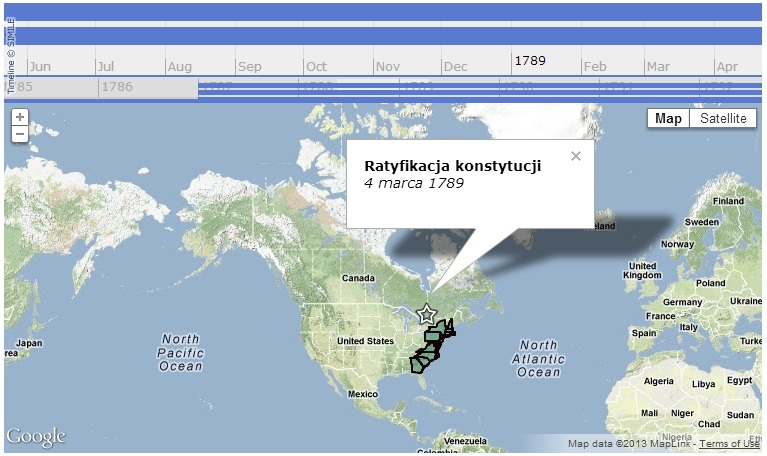
\includegraphics[width=100mm]{ge/st1.jpg}
  \caption{Rok 1789.}
  \label{fig:st1}
\end{figure}

Kolejny rysunek ukazuje aktualny stan granic. Widać że utrzymuje się on od 1959 roku.

\begin{figure}[H]
  \centering
    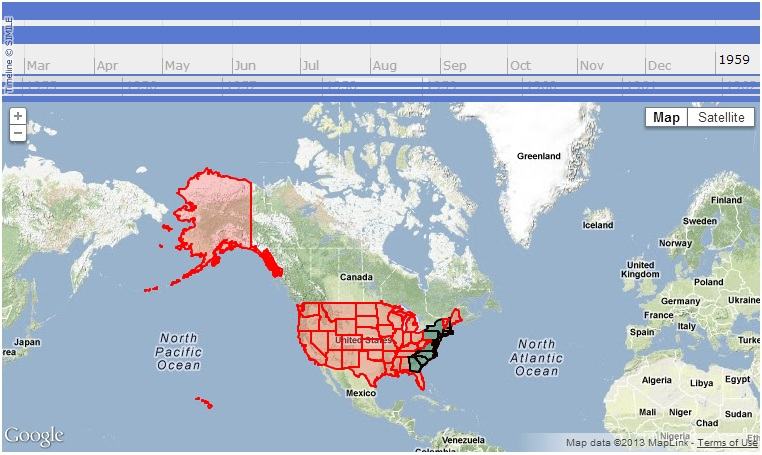
\includegraphics[width=100mm]{ge/st3.jpg}
  \caption{Rok 1959.}
  \label{fig:st3}
\end{figure}

\section{Granice Polski i Rzeczpospolitej Obojga Narodów}
\label{sec:usahistory}

Kolejny przykład przedstawia możliwość zmiany rodzaju danych w zależności od stopnia przybliżenia. Rysunek \ref{fig:po1} przedstawia granice wytyczone przy pomocy funkcji tworzącej linie bezier-a. Przy tak dużym oddaleniu szczegóły rysunku nie są widoczne, nie można przekazać wielu szczegółów.

\begin{figure}[H]
  \centering
    \includegraphics[width=100mm]{ge/polska-teraz.png}
  \caption{Polska obecnie.}
  \label{fig:po1}
\end{figure}

W prosty sposób można określić ogólne granice w dowolnym punkcie w czasie. Poniższy rysunek przedstawia wynik obszaru który został określony przez 105 punktów.

\begin{figure}[H]
  \centering
    \includegraphics[width=100mm]{ge/polska-ron.png}
  \caption{Polska w roku 1691.}
  \label{fig:po2}
\end{figure}

W celu dostarczenia większej ilości informacji, możliwe jest załączenie pliku graficznego, w tym przypadku jest to zdjęcie mapy która przedstawia dokładny obszar Rzeczpospolitej Obojga Narodów. Jeszcze bliższe przybliżenie pozwali na odczytanie nazw miejscowości i obszarów geograficznych. 

\begin{figure}[H]
  \centering
    \includegraphics[width=100mm]{ge/polska-ron-map.png}
  \caption{Rzeczpospolita Obojga Narodów, mapa.}
  \label{fig:po3}
\end{figure}

\chapter{Podsumowanie}

Wysoki rozwój techonologi komputerowerj pozwala na redefiniowanie pojeć znanych człowiekowi od długiego czasu. Niniejsza praca udowania tą tezę, mapa która od zawsze była tylko niezmienną, graficzną repreznetacją terenu przy wykorzystaniu nowoczesnych technologi może stać się interatktywnym obiektem pozwalającym na ukazanie niedostępnych wcześniej danych w zupełnie nowy sposób.

Główna technologia wybrana do tworzenia aplikacji wykorzystywanej w przeglądarkach internetowych posiadającą możliwość interakcji użytkownika z danymi powinna dawać możliwość aktualizacji jedynie wybranych fragmentów danych, tak aby wyeliminować zbędne renderowanie stałych fragmentów. W takim przypadku dobrym wyborem jest JavaScript który dzięki założenion postawionym podczas jego tworzenia idealnie sprawdza się w tego typu zadaniach.

Format zapisu danych powinien zapewniać obsługę zawórno dowolnych punktów na kuli ziemskiej jak i dodatkowych elementów które mogą być dołączone go wejściowego zbioru danych. Ogólnodostępny format WGS pozwala na proste przechowywanie informacji o położeniu obiektów, jego zapis jest zarówno czytelny dla człowieka jak i dla komputera. Wybrany format zapisu plików, GML, pozwala na łatwe przechowaywanie niemal wszystkich informacji w jednym miejcu, jedynie obrazy graficzne wymagają podania ścieżki do ich fizycznej lokalizacji.

Wybór Google Maps jako podstawowe źródło informacji geograficznych, dostarczających statyczny obraz map dało dostęp do ogromnej bazy danych. Niestety najnowsze rozwiązania nie zawsze zapewniają kompatybilność ze starszymi, przykładem jest jeden z elementów HTML w wersji 5, canvas. Jego wykorzystanie okazało się niemowżliwe w połączeniu wybranymi mapami których interfejs został stworzony bez możliwości ich wykorzystania. Zaawansowaną grafikę udało się stworzyć przy pomocy SVG, formatu który nawet skompliwoany obraz potrafi zapisać w zwięzłej i krókiej formie oszczędzając miejsce na dysku przy zachowaniu szczegółowości i ilości detali. Stworzone algorytmy do stopniowego generowania obiektów i ich zmiany w zależniości od atrybutów mapy pozwalają na minimalizowanie wymagań w odniesiu do procesora i szybsze dostarczanie wartościowych danych.

Zwrócono również uwagę na bezpieczeństwo tworzonego projektu. Powstała aplikacja jest niezależna od jakichkolwiek zewnętrznych baz danych, dlatego ewentualna kontrola dostępu jest wykonywana przez nadrzędną wartstę którą jest serwis używający map. Kontrola poprawności danych jest możliwa dzięki wykorzystaniu funkcji tworzących sumę kontrolną, użytkownik może dokonać jej porównania z wartością do której autentyczność jest niezaprzeczalna. Taka czynność daje pewność że dane które posiada użytknownik są poprawne i stworzone przez autoryzowane osoby.

Zastosowane metody optymalizacji framework-u pozwoliły na zwięszenie płynności działania, jedynie niezbędne akcje są wykonywane podczas jego pracy. Operacje zbędnę, lub takie które mogą zostać wykonane w późniejszym czasie są zatrzymwane i uruchamiane jedy gdy jest to niezbędne.

Podsumowując stworzona aplikacja spełnia wszelkie warunki aby można było ją uznać za użyteczną podczas procesu nauki. Posiada intuicyjny interejs pozwalający na łatwą obsługę, dostarcza cennych informacji a szeroki zakres prezentacji danych, możliwość tworzenia płynnych przejśc kształtów, kolorów sprawia że jest interesująca i przyciąga uwagę użytkownika. Wykorzystanie jej m.in. na lekcji histori pozwoli zmienić statyczne reprezentacje ruchów wojennych w ciekawe i interaktywne, taka forma może zwiększyć przyswajalność widzy i zachęcić do czestych powtórek poza salą lekcyjną.



\appendix
\chapter{Dodatek A}
\label{cha:appa}

\section{Oryginalny plik kml}
\label{sec:akml}

\lstset{language=XML}
\begin{lstlisting}[caption=caption]
<?xml version="1.0" encoding="UTF-8"?>
<kml>
  <Document>
    <name><![CDATA[US States]]></name>
    <open>1</open>
    <Style id="Style_5">
      <LabelStyle>
        <color>9900ffff</color>
        <scale>1</scale>
      </LabelStyle>
      <LineStyle>
        <color>990000ff</color>
        <width>2</width>
      </LineStyle>
      <PolyStyle>
        <color>997f7fff</color>
        <fill>1</fill>
        <outline>1</outline>
      </PolyStyle>
    </Style>
    <Placemark id="pm251">
      <name><![CDATA[Hawaii (1959)]]></name>
      <Snippet maxLines="0">empty</Snippet>
      <description></description>
      <TimeSpan>
        <begin>1989</begin>
      </TimeSpan>
      <styleUrl>#Style_5</styleUrl>
      <MultiGeometry>
        <MultiGeometry>
          <Polygon id="g867">
            <altitudeMode>clampToGround</altitudeMode>
            <outerBoundaryIs>
              <LinearRing>
                <coordinates>
-159.335174733889,21.9483433404175
-159.327130348878,22.0446395507162
-159.295025589769,22.1248124949548
-159.343195828355,22.1970166285359
-159.391366885913,22.2291198667724
-159.576012589057,22.2131796383001
-159.712505933171,22.1490592515515
-159.800814224332,22.0366665967853
-159.736592652746,21.9644203111023
-159.640246973766,21.9483657695954
-159.576021285803,21.8841361312636
-159.439545188912,21.8680716835921
-159.335174733889,21.9483433404175
                </coordinates>
              </LinearRing>
            </outerBoundaryIs>
          </Polygon>
        </MultiGeometry>
      </MultiGeometry>
    </Placemark>
  </Document>
</kml>

\end{lstlisting}

\section{Zapis w pamięci sesyjnej}
\label{sec:ass}

\lstset{language=XML}
\begin{lstlisting}[caption=caption]
[{"start":"1989","end":"2010","polygon":[{"lat":21.9483433404175,"lon":-159.335174733889},{"lat":22.0446395507162,"lon":-159.32713034887797},{"lat":22.1248124949548,"lon":-159.295025589769},{"lat":22.1970166285359,"lon":-159.34319582835496},{"lat":22.2291198667724,"lon":-159.391366885913},{"lat":22.2131796383001,"lon":-159.57601258905697},{"lat":22.1490592515515,"lon":-159.71250593317097},{"lat":22.0366665967853,"lon":-159.800814224332},{"lat":21.9644203111023,"lon":-159.73659265274603},{"lat":21.9483657695954,"lon":-159.640246973766},{"lat":21.8841361312636,"lon":-159.576021285803},{"lat":21.8680716835921,"lon":-159.439545188912},{"lat":21.9483433404175,"lon":-159.335174733889}],"title":"Hawaii (1959)","mId":"pm251","pId":"g867","color":"#ff0000","width":2,"opacity":0.59765625,"fillcolor":"#ff7f7f","name":"Hawaii (1959)","desc":""}]
\end{lstlisting}

\section{Wynik końcowy}
\label{sec:aresult}

\begin{figure}[H]
  \centering
    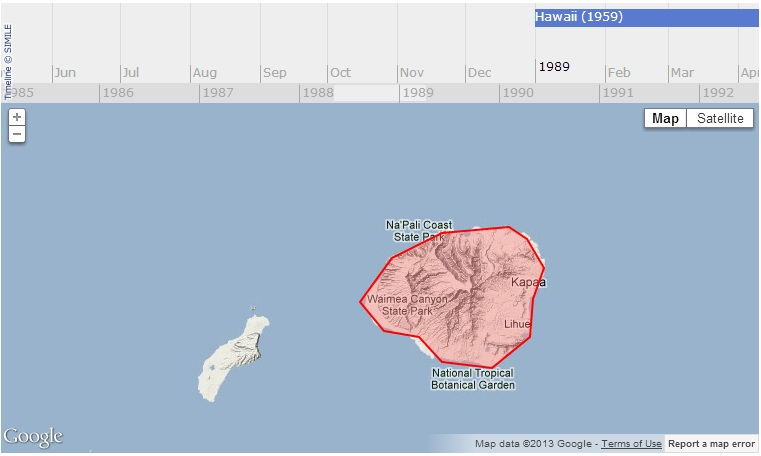
\includegraphics[width=100mm]{ge/hawaii.jpg}
  \caption{Hawaje}
  \label{fig:hawaii}
\end{figure}

\pagebreak[4]
\listoffigures
\pagebreak[4]
\listoftables

\bibliographystyle{alpha}
\bibliography{bibliografia}

\end{document}
